\documentclass{article}

\usepackage{fancyhdr}
\usepackage{extramarks}
\usepackage{amsmath}
\usepackage{amsthm}
\usepackage{amsfonts}
\usepackage[plain]{algorithm}
\usepackage{algpseudocode}
\usepackage{matlab-prettifier}
\usepackage{graphicx}
\usepackage[export]{adjustbox}
%
% Basic Document Settings
%
\lstMakeShortInline[style=Matlab-editor]"

\topmargin=-1in
\evensidemargin=0in
\oddsidemargin=0in
\textwidth=6.5in
\textheight=9.0in
\headsep=0.25in

\linespread{1.1}


\rhead{\firstxmark}
\lfoot{\lastxmark}
\cfoot{\thepage}

\renewcommand\headrulewidth{0.4pt}
\renewcommand\footrulewidth{0.4pt}

%
% Homework Details
%   - Title
%   - Due date
%   - Class
%   - Section/Time
%   - Instructor
%   - Author
%

\newcommand{\hmwkTitle}{AMATH 482 Homework 5 : Background Subtraction in Video Streams}
\newcommand{\hmwkDueDate}{March 15, 2019}
\newcommand{\hmwkClassInstructor}{Professor Nathan Kutz}
\newcommand{\hmwkAuthorName}{\textbf{Skyler Hallinan}}

%
% Title Page
%

\title{
    \textmd{\textbf{\text{ } \hmwkTitle}}\\
}

\author{\hmwkAuthorName}
\date{}

\begin{document}
\maketitle

\section*{\fontsize{19}{15}\selectfont Abstract}
		We recorded several videos with a foreground object and a background object (a student (object) walking in various locations (background)), with subtle variations in each video, such as distance from object to the camera, as well as amount of noise in the data. We used the dynamic mode decomposition to separate the foreground and background from the videos, truncating our matrices by looking at energies captured by singular values. We also looked at the omega values from these decompositions to see how much of the background we were capturing with additional modes. We were able to successfully separate foreground and background from five different videos, even with high noise levels.
\section*{\fontsize{19}{15}\selectfont Introduction and Overview}
	We can think of complex systems as high-dimensional, nonlinear dynamical systems that exhibit many phenomena in both space and time. Even though these systems are complex, they can often by represented by low-dimensional spatio-temporal coherent structures. The dynamic mode decomposition allows us to discover dynamical systems from this otherwise high-dimensional data. It is equation-free and based on the underlying data; it's output, the decomposition of complex data into spatio-temporal coherent structures, is practical and useful. At the same time, it is simple, fast to execute (cost of algorithm is SVD), and does not make underlying assumptions about the data. At the core, the dynamic mode decomposition is a combination of spatial-dimensionality reduction techniques such as singular value decomposition and proper orthogonal decomposition and Fourier transforms in time. \\ \\
	We have recorded a set of five videos to analyze. The dynamic mode decomposition relies on having snapshots of data at $k$ points in time from a dynamical system; each frame in our video represents this data at each $t_k$. We will use the dynamic mode decomposition to separate the foreground from the background in our videos. We used a laptop to record our videos so that we could have a stable camera so that our background could be free of noise, and so that we could easily separate our foreground and background. These five videos have different levels of noise, distance from the foreground to background, and color difference between background and foreground. \\ \\ 
	The dynamic mode decomposition will return a low-rank approximate reconstruction of our data, which will represent the background of our video. By subtracting this low-rank approximation from the original data, we will be able to get the sparse reconstruction, which will represent the foreground object. Finally, we will use a residual matrix "R" to remove negative pixel values from our sparse matrix and compensate the low-rank matrix and sparse matrix accordingly.
\section*{\fontsize{19}{15}\selectfont Theoretical Background}
	The DMD, given a dynamical system and two sets of data $X$ and $X'$ where $\mathbf{x}_{k}^{\prime}=\mathbf{F}\left(\mathbf{x}_{k}\right)$ such that F is a map corresponding to time evolution, finds the eigendecomposition of the best-fit linear operator $A$ where $\mathbf{X}^{\prime} \approx \mathbf{A X} \Rightarrow \mathbf{A}=\mathbf{X}^{\prime} \mathbf{X}^{\dagger}$ As a result, the DMD modes are the eigenvectors of A, and each DMD mode corresponds to a particular eigenvalue (of A). This solution minimizes the error $\left\|\mathbf{X}^{\prime}-\mathbf{A} \mathbf{X}\right\|_{F}$ where $||\cdot||_F$ is the Frobenius norm denoted by $\|\mathbf{X}\|_{F}=\sqrt{\sum_{j=1}^{n} \sum_{k=1}^{m} X_{j k}^{2}}$. It does this by constructing an approximate locally linear dynamical system $\frac{d \mathbf{x}}{d t}=\mathcal{A} \mathbf{x}$ with initial condition $x(0)$ and solution of $\mathbf{x}(t)=\sum_{k=1}^{n} \phi_{k} \exp \left(\omega_{k} t\right) b_{k}=\Phi \exp (\Omega t) \mathbf{b}$, where $\phi_k$ and $\omega_k$ are the eigenvectors and eigenvalues of the matrix A, and $b_k$ is the coordinates of x(0) in the eigenvector basis. We solve  $\mathrm{A}=\exp (\mathcal{A} \Delta t)$ with $\mathbf{x}_{k}=\sum_{j=1}^{r} \boldsymbol{\phi}_{j} \lambda_{j}^{k} b_{j}=\boldsymbol{\Phi} \Lambda^{k} \mathbf{b}$, minimizing the least-squares trajectory of $x_k$. \\ \\
	The DMD approximates modes of the Koopman operator, a linear, infinite-dimensional operator that is a ''nonlinear dynamical system on the Hilbert space of measurement functions of the states''. This Koopman operator advances measurements along with the flow map $F$ as shown below. 
\begin{align*}
K\ g &=g \circ \mathrm{F} \\ 
\Longrightarrow \quad K\ g\left(\mathbf{x}_{k}\right) &=g\left(\mathbf{F}\left(\mathbf{x}_{k}\right)\right)=g\left(\mathbf{x}_{k+1}\right)
\end{align*}
	The data needed for dynamical mode decomposition (DMD) is that from a dynamical system $\frac{d \mathbf{x}}{d t}=\mathbf{f}(\mathbf{x}, t ; \mu)$ where $\mathbf{x}(t) \in \mathbb{R}^{n}$ is a vector that represents the state of our dynamical system at time $t$, $\mu$ represents parameters of the system, and $f(\cdot)$ represents the dynamics. We can represent the continuous-time dynamics from the previous equation as a corresponding discrete-time representation where we sample at $\Delta t$ and denote the time in the equation as  $\mathbf{x}_{k}=\mathbf{x}(k \Delta t)$. Then, we have a discrete-time flow map described by $\mathbf{x}_{k+1}=\mathbf{F}\left(\mathbf{x}_{k}\right)$ and $\mathrm{y}_{k}=\mathrm{g}\left(\mathrm{x}_{k}\right)$ at $t_k$ values where  $k = 1,2,...n$ for n different times. The measurements equal the states in many applications, that is, $y_k = x_k$. In addition, our initial conditions are $x(t_0) = x_0$. Thus we have a set of governing equations and an initial condition. We represent our data into two large snapshots $X$ and $X'$, where $X$ is the column-wise data from $x_1$ to $x_{m-1}$ and $X'$ is the column-wise data from $x_2$ to $x_m$ such that $\mathrm{X}^{\prime} \approx \mathrm{AX}$ and so that we can calculate the best-fit $A$ matrix via the pseudo inverse  $\mathbf{A}=\mathbf{X}^{\prime} \mathbf{X}^{\dagger}$, which minimizes the error as stated above. We assume this data is high-dimensional so the size of our snapshot is much larger than the number of snapshots. This allows us to project our data onto POD modes to solve for A without explicitly computing it.\\ \\
We calculate the DMD in the following way: We first take the singular value decomposition of $X$ such that $\mathrm{X}=\mathrm{U} \Sigma \mathrm{V}^{*}$, where $U \in \mathbb{C}^{n \times r}, \Sigma \in \mathbb{C}^{r \times r}, \mathbf{V} \in \mathbb{C}^{m \times r}$, and we define $r$ to be the rank of the reduced SVD approximation of X. We then determine the matrix A from earlier  by computing the $r\times r$ projection of $A$ onto POD modes via $\tilde{\mathrm{A}}=\mathrm{U}^{\prime} \mathrm{AU}=\mathrm{U} \mathrm{X}^{\prime} \mathrm{V} \Sigma^{-1}$. We see that this $\tilde{A}$ defines the low-dimensional linear model of our dynamical system on POD coordinates: $\tilde{\mathbf{x}}_{k+1}=\tilde{\mathbf{A}} \tilde{\mathbf{x}}_{k}$. Next, we calculate the eigendecomposition of $\tilde{A}$, with $\tilde{\mathrm{A}} \mathrm{W}=\mathrm{W} \Lambda$, where our $W$ columns represent eigenvectors and $\Lambda$ contains a diagonal matrix of our eigenvalues. Finally, we reconstruct the eigendecomposition by creating a matrix where the columns represent exact DMD modes: $\Phi=\mathbf{X}^{\prime} \mathbf{V} \Sigma^{-1} \mathbf{W}$. We can then, afer declaring  $\omega_{k}=\ln \left(\lambda_{k}\right) / \Delta t$, project the future solution at times in the future using: $\mathbf{x}(t) \approx \sum_{k=1}^{r} \phi_{k} \exp \left(\omega_{k} t\right) b_{k}=\Phi \exp (\Omega t) \mathbf{b}$. This can be interpreted as the least-square fit/regresion of a best-fit linear dynamical system $\mathbf{x}_{k+1}=\mathbf{A} \mathbf{x}_{k}$. Once again, this is constructed so that we minimize the norm $\left\|\mathrm{x}_{k+1}-\mathrm{Ax}_{k}\right\|_{2}$ across all timepoints/snapshots. Finally, we calculate the initial coefficient values $b_k$ by considering our initial snapshot $x_1$ at time $t_1 = 0$. Solving, we find the pseudo inverse (since the eigenvector matrix is not square) to get our $b$:  $\mathbf{b}=\mathbf{\Phi}^{\dagger} \mathbf{x}_{1}$\\ \\
We see that we can use the DMD spectrum of frequencies to subtract background modes. We create two data frames from our initial: One from the beginning to the $last-1$ frame, and one from the 2nd to $last$ frame, where each of these represent a data snapshot: the data matrix $X$, and the shifted data matrix $X'$ . We use the first data frame for our SVD and corresponding analysis. We assume that $\omega_{p},$ where $p \in\{1,2, \ldots, \ell\},$ satisfies $\left\|\omega_{p}\right\| \approx 0,$ and that $\left\|\omega_{j}\right\| \forall j \neq p$ is bounded away from zero, giving us the following: 
\begin{align*}
\mathrm{X}_{\mathrm{DMD}}=\underbrace{b_{p} \varphi_{p} e^{\omega_{p} t}}_{\text { Background Video }}+\underbrace{\sum_{j \neq p} b_{j} \varphi_{j} e^{\omega_{j} t}}_{\text { Foreground Video }}
\end{align*}
This will produce a $X_{DMD}$ matrix the same dimensions as our original $X$ matrix, although each term is complex. We will solve for the various parameters using the procedure outlined previously. \\ \\
After we get this DMD matrix $\mathbf{X}_{\mathrm{DMD}}^{\text { Low-Rank }}=b_{p} \varphi_{p} e^{\omega_{p} t}$, since, we know $\mathbf{X}=\mathbf{X}_{\mathrm{DMD}}^{\mathrm{Low}-\mathrm{Rank}}+\mathbf{X}_{\mathrm{DMD}}^{\mathrm{Sparse}}$, we can solve for the sparse matrix $\mathbf{X}_{\mathrm{DMD}}^{\text { Sparse }}=\sum_{i \neq n} b_{j} \varphi_{j} e^{\omega_{j} t}$ via  $\mathbf{X}_{\mathrm{DMD}}^{\mathrm{Sparse}}=\mathbf{X}-\left|\mathbf{X}_{\mathrm{DMD}}^{\mathrm{Low}-\mathrm{Rank}}\right|$.  
Finally, with these low-rank and sparse DMD approximations, of the image, since we subtracted the low-rank approximation from our initial data to obtain our sparse approximation reconstruction, we may obtain negative values in our sparse matrix. This does not make sense because pixel values cannot be negative. We put these negative values into a residual $n\times m$ matrix $R$ and then create our low-rank and sparse reconstructions as follows: 
\begin{align*}
\mathbf{X}_{\mathrm{DMD}}^{\mathrm{Low}-\mathrm{Rank}} \leftarrow \mathbf{R}+\left|\mathbf{X}_{\mathrm{DMD}}^{\mathrm{Low}-\mathrm{Rank}}\right| \\
\mathbf{X}_{\mathrm{DMD}}^{\mathrm{Sparse}} \leftarrow \mathbf{X}_{\mathrm{DMD}}^{\mathrm{Sparse}}-\mathbf{R}
\end{align*}
This allows us for us to account for the magnitudes of complex values from the DMD reconstruction, while preventing pixel intensities from being below zero, making sure that both approximate low-rank and sparse DMD reconstructions are real-valued, and maintaining that $\mathbf{X}=\mathbf{X}_{\mathrm{DMD}}^{\mathrm{Low}-\mathrm{Rank}}+\mathbf{X}_{\mathrm{DMD}}^{\mathrm{Sparse}}$. Adding these "R" values back will not necessarily make our DMD better at separating foreground and background, but it will make sure that we have the non-negative conditions that we discussed earlier.
\\ \\ The DMD is a way to make a low-rank approximation of linear maping that approximate the nonlinear dynamics of a given system. It is simple and equation-free, and can be used for future state prediction for any time $t$. The DMD does have its limitations. Like PCA, it is based on a singular value decomposition that extracts correlated patterns from the data. Like SVD, it cannot handle efficiently handle invariances in the data. Translational and rotational invariances as well as transient time phenomena are not characterized well by SVD and therefore DMD. 
\section*{\fontsize{19}{15}\selectfont Algorithm Development}
We used "VideoReader" to create a "vid" object to load in our mp4 videos. We created a $dt$ using $\frac{1}{\text{Framerate}}$ of the loaded video, and a time vector by spacing from 0 to the "Length" of the video in intervals of "dt". Using a loop similar to the one used in Homework 3, we loaded in each frame of the video. We converted this image matrix to grayscale (to allow us to do computation on it) using "rgb2gray" and converted its values to double (from uint8). To reduce computational time needed, we scaled the image down by a factor of $\frac{1}{4}$ using "imresize" so that the final image was $180\times320$. We used "reshape" to convert this into a column, and added it to our data matrix. We repeated this at all time points, effectively creating a data matrix where each column represented a grayscale image at a specific point in time, in chronological order from left to right. \\ \\
	Next, we split this data matrix into two data matrices, "X1" and "X2" , where X1 represented the snapshots of data from frame 1 to the last -1 frame, while the second matrix represented the data from snapshot frame 2 to the last frame. We created these two vectors this way because our goal was to determine how to get from one snapshot "X1" to the next snapshot "X2" using some linear transformation "A", and these could be approximations of $X$ and $X'$. We then took the singular value decomposition of "X1" using "svd(X1)". We plotted the diagonal values of the "s" matrix using "diag" divided by the sum of the diag values to see how much energy each singular value could capture in this system. We looked at this graph and determined how many significant modes there were, that is, how many modes that captured a significant proportion of the energy of the system, and saved this value as "r". \\ \\
We then truncated our "u", "s", and "v" matrices from our "svd" to contain only 1:"r" of its original row or column values (For example, we set "U = u(:,1:r)"), effectively only pulling out "r" modes from these dataframes. We then transformed to the low-rank domain by constructing a new variable "Atilde" which was equal to "U_r' * X2 * V_r / S_r". We took the eigen value decomposition of "Atilde" using "[W,D] eig" to get its eigen vectors and eigen values. This was essentially taking the approximate low-rank subspace "Atilde" and doing an eigen decomposition to diagonalize frequencies. We created our DMD modes using "Phi = X2 * V_r / S_r * W_r", and looked at the spectra modes by finding the eigen values (by taking the "diag" eigen values "D" matrix). We were able to obtain our "omega" values by taking the log of these eigen values and dividing them by our "dt". We then plotted these (after determining an ideal number of modes to use). \\ \\ 
We then calculated our DMD solution. We set our initial condition to be the first frame of our "X1" matrix (the first column). We then solved for our "b" value using "b= Phi\ x1". We then created an empty "zeros" matrix of size "(r, length(t))", and iteratively created a time dynamics matrix, which we populated at each time point using "(b.*exp(omega*t(iter)))". We then multiplied "Phi" by this time dynamics matrix to get our low-rank DMD approximation "Xdmd". \\ \\ 
Our original data matrix "X1" is the sum of the low-rank and the sparse matrix approximations, so we subtracted "Xdmd" from "X1" to get our sparse DMD reconstruction approximation. We then created our R matrix to account for the residual negative values of our sparse matrix. We did this by filtering our sparse matrix so that it only contained the negative values, and we set "R" to this. To make a more accurate low-rank DMD and sparse DMD approximation, we added "R" to the absolute value "abs" of our low rank matrix to get our final low-rank DMD approximation. To get our final sparse DMD approximation, we subtracted "R" from our original sparse matrix. \\ \\ 
We then arbitrarily picked a frame number, and took one column from the sparse matrix, the low-rank matrix, the sparse - "R" matrix, the "abs("low-rank") + R" matrix, the original data matrix "X1", and the "X" total reconstruction of low-rank + sparse.  We reshaped this column, which corresponded to an image at a time point, into an image, and used "imshow" to visualize how they were different. We also used "implay" to compare the entire matrices by playing them as videos, but we did not include those in this paper. We repeated the above steps for all five videos.
\section*{\fontsize{19}{15}\selectfont Computational Results}
\begin{figure}[H]
\begin{center}
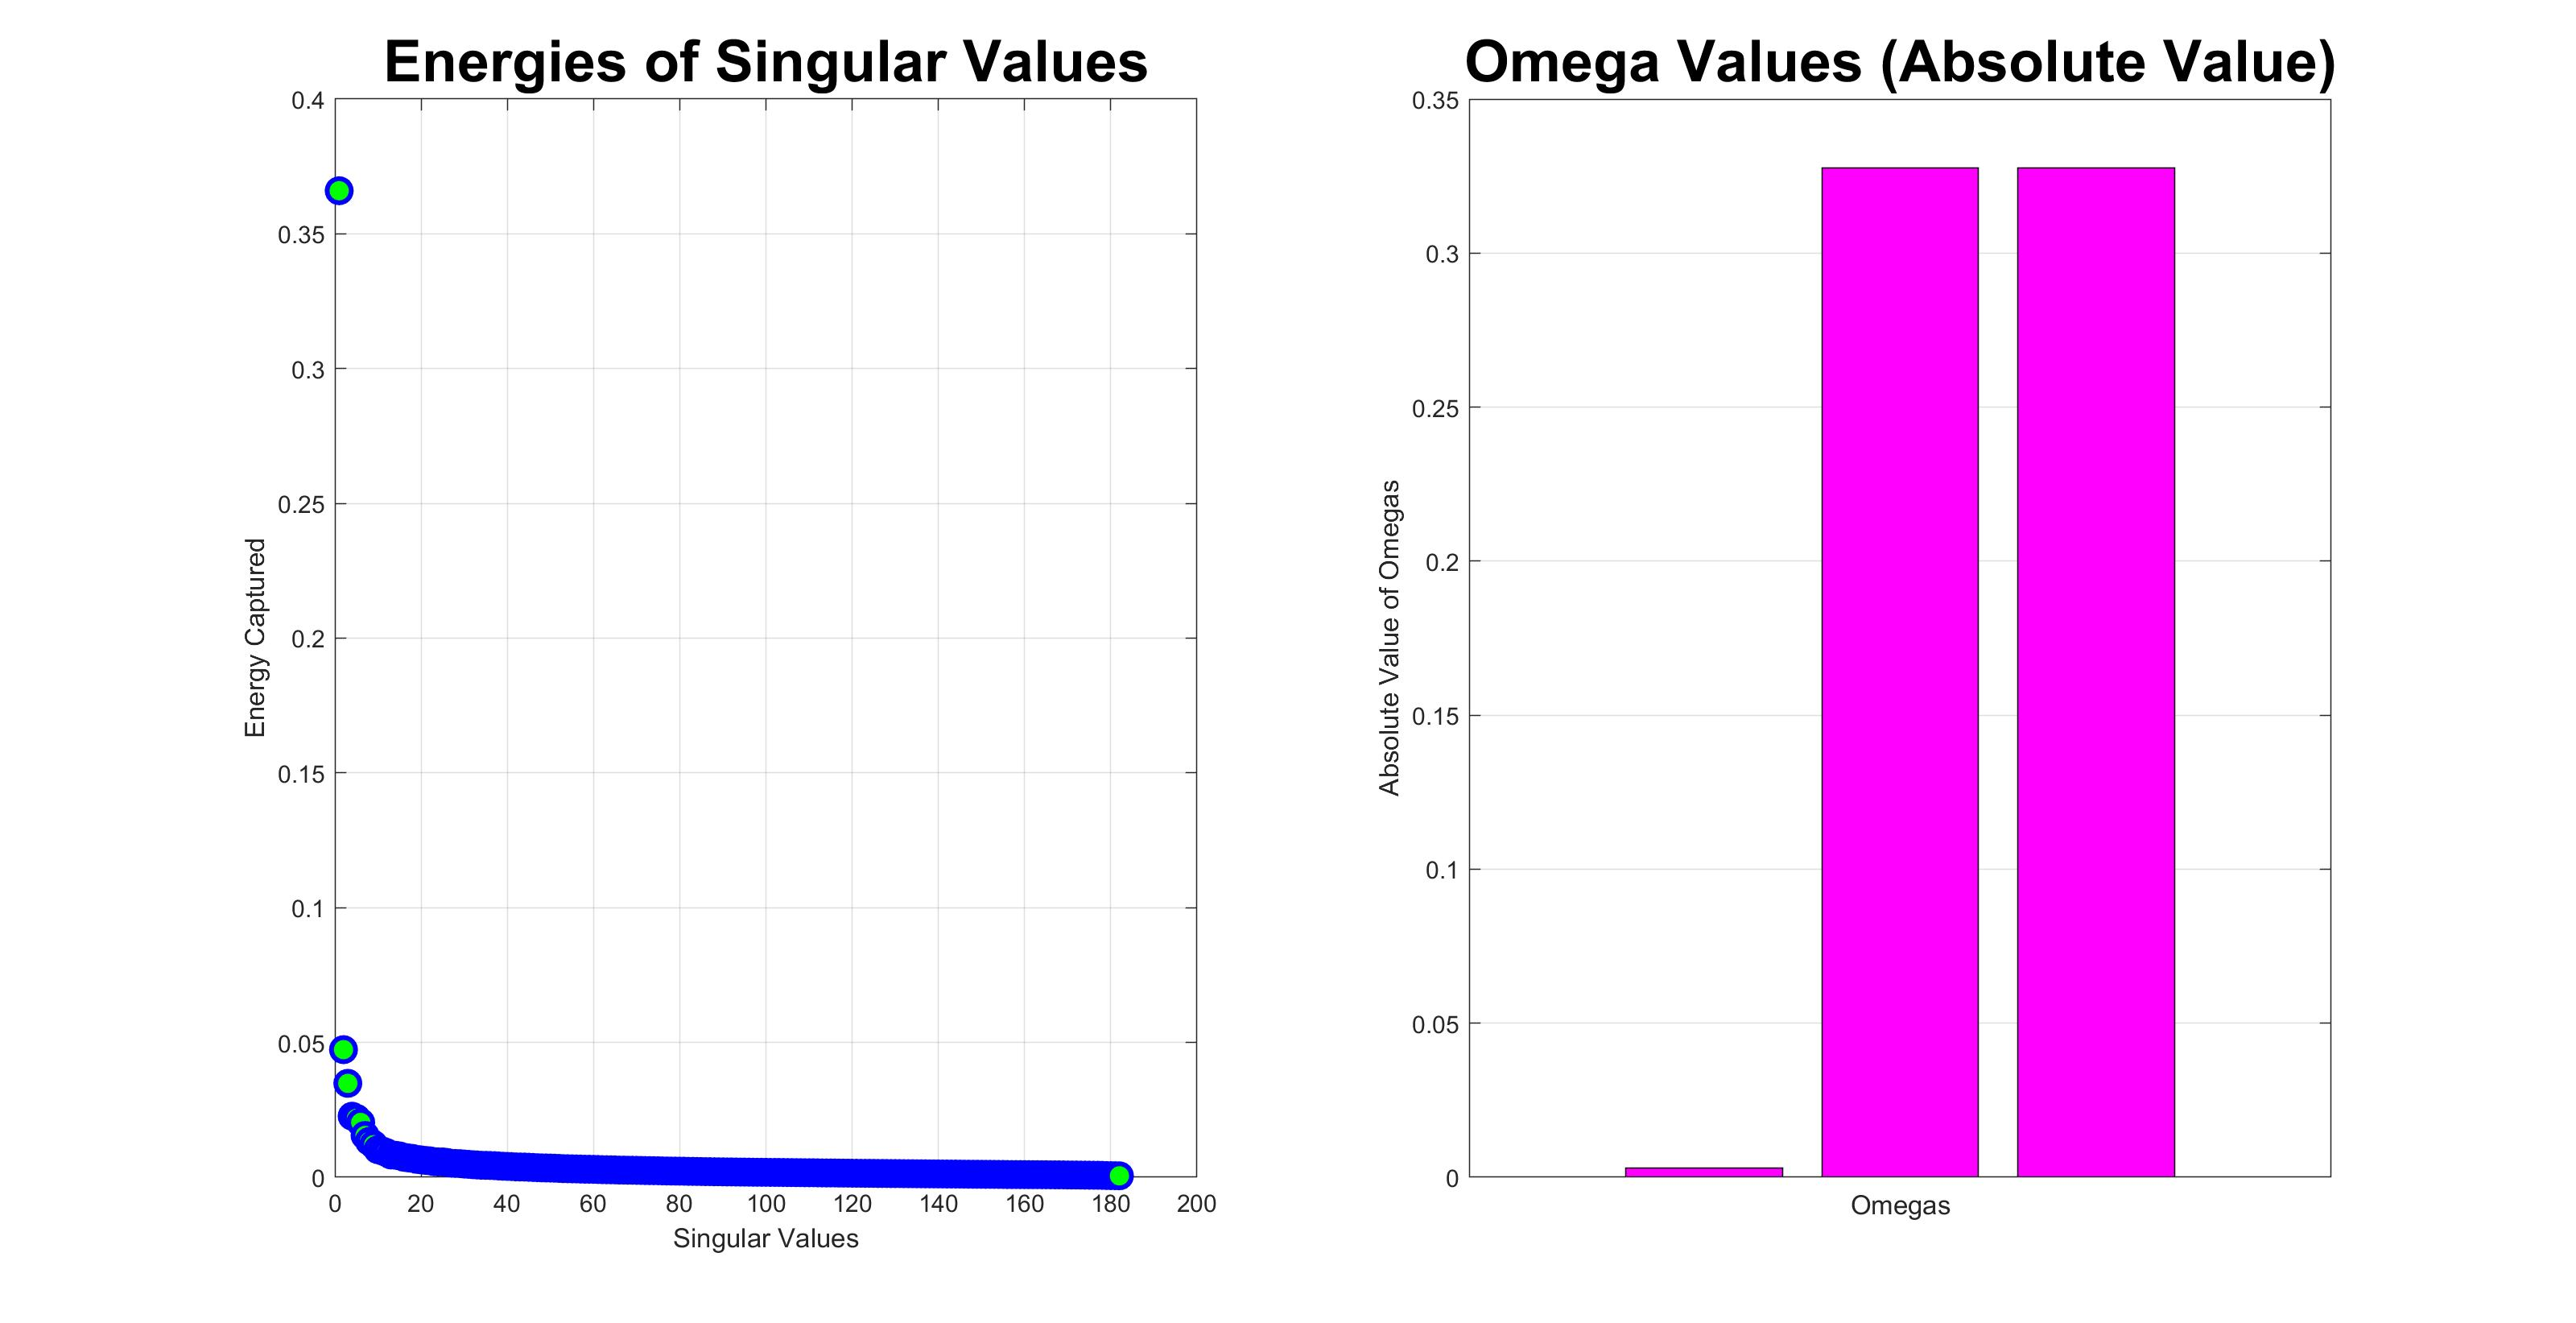
\includegraphics[width = 12cm]{energy1}
\caption{\label{fig:scaled_diss} Plots of (normalized) energy captured by singular values (left) and omega values (right) (Video 1)}
\end{center}
\end{figure}
\begin{figure}[H]
\begin{center}
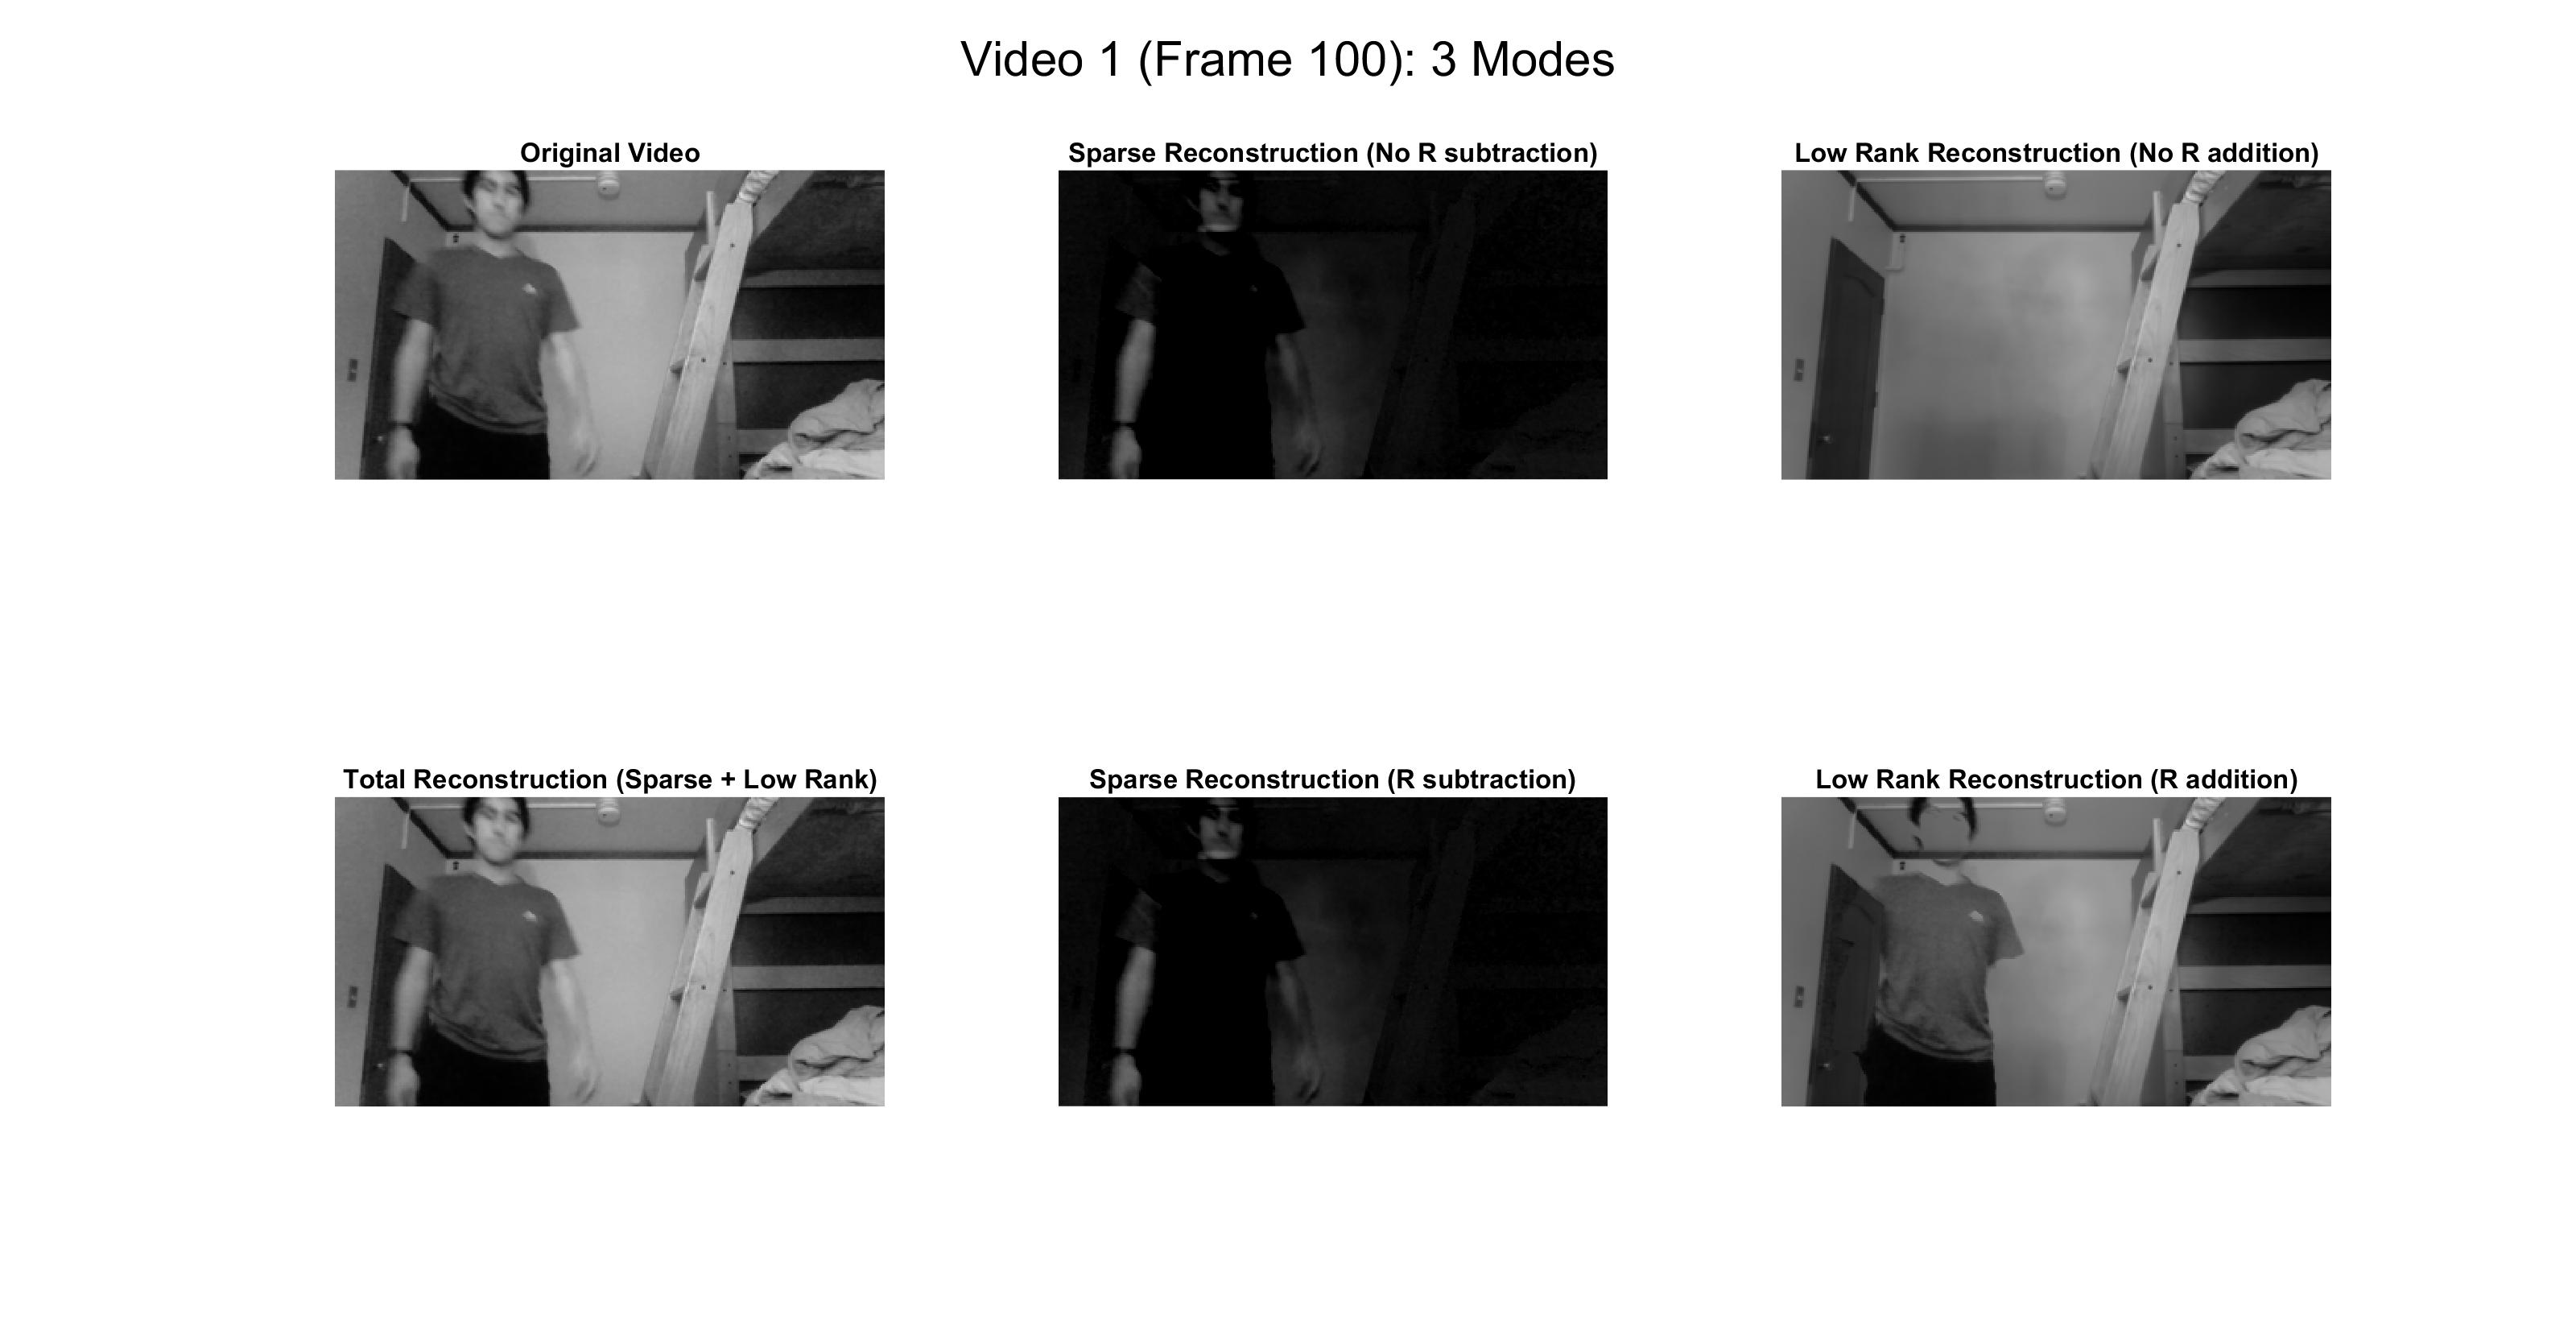
\includegraphics[width = 16cm]{vid1image}
\caption{\label{fig:scaled_diss} Video separation and reconstruction (Video 1)}
\end{center}
\end{figure}
\textbf{Video 1: Ideal Case} \\
In this video, we recorded from the laptop that was sitting on a laptop, to hold a background constant. The background object was the ladder and wall of a dorm room, while the foreground object was a student walking throughout the room at various distances. \\ \\
We see that our energy diagram of the singular values  (Figure 1) shows that about three modes are significant. We set our "r" value to be 3, so we truncated our "u", "s", and "v" matrices from 1:3 from "svd(X1)" and calculated the low-rank approximation. We also see that the absolute value of our first "omega" value is extremely close to 0, while the next two are a bit higher. The "omega" close to 0 indicates that it is a background mode. We see that although we used an "r = 3", that is, we assumed three significant modes to determine our background DMD low-rank matrix, we could probably achieve similar results using only one mode. This is something that we computationally tested and determined to be true. \\ \\
From Figure 2, we see that our sparse reconstruction, which should show the foreground, looks relatively similar for both cases where we incorporated our "R" matrix and when we did not. In both cases, the foreground (the student) is relatively visible and is clearly separated from the background. In terms of the low-rank reconstruction, the background, adding "R" seems to have made the DMD reconstruction worse. There is a definite presence of the object (the student) in the form of floating clothes, although some of the foreground object is now transparent. We see however that the low-rank reconstruction that does not use "R" does a great job of only showing the background. Finally, our total reconstruction, which is the sum of the low rank and the sparse approximations, gave us an image that looked like the original video. Thus, our DMD separation has worked.
\begin{figure}[H]
\begin{center}
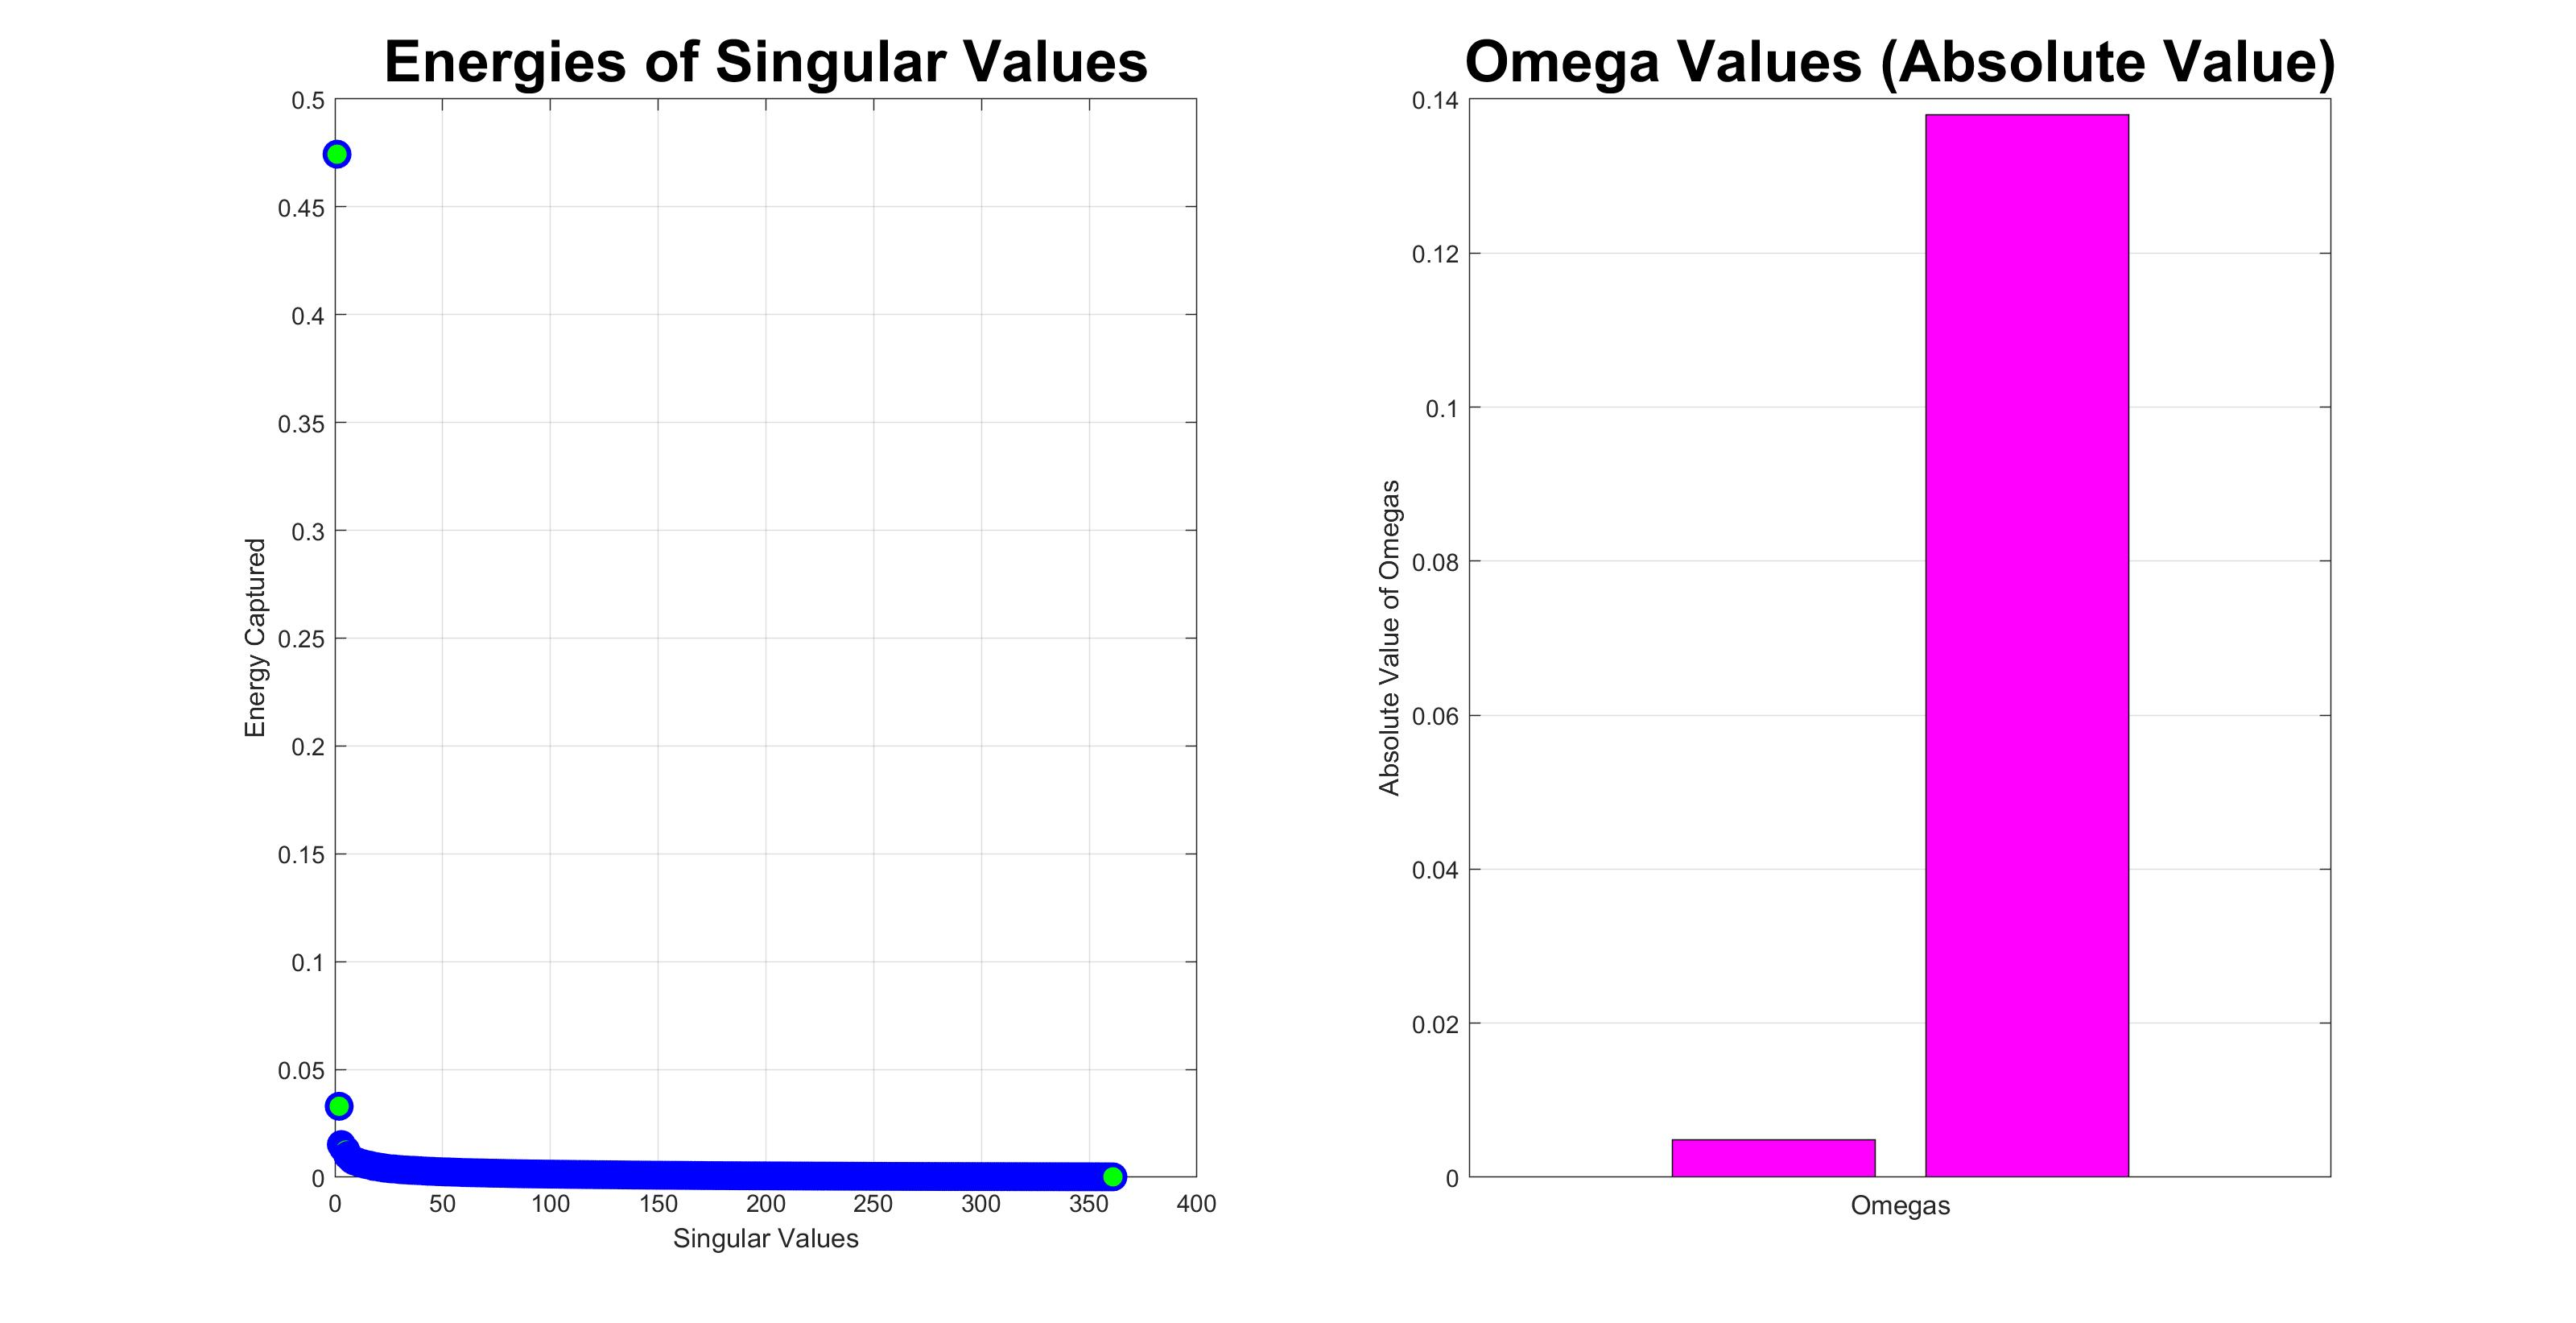
\includegraphics[width = 12cm]{energy2}
\caption{\label{fig:scaled_diss} Plots of  (normalized) energy captured by singular values (left) and omega values (right)(Video 2)}
\end{center}
\end{figure}
\begin{figure}[H]
\begin{center}
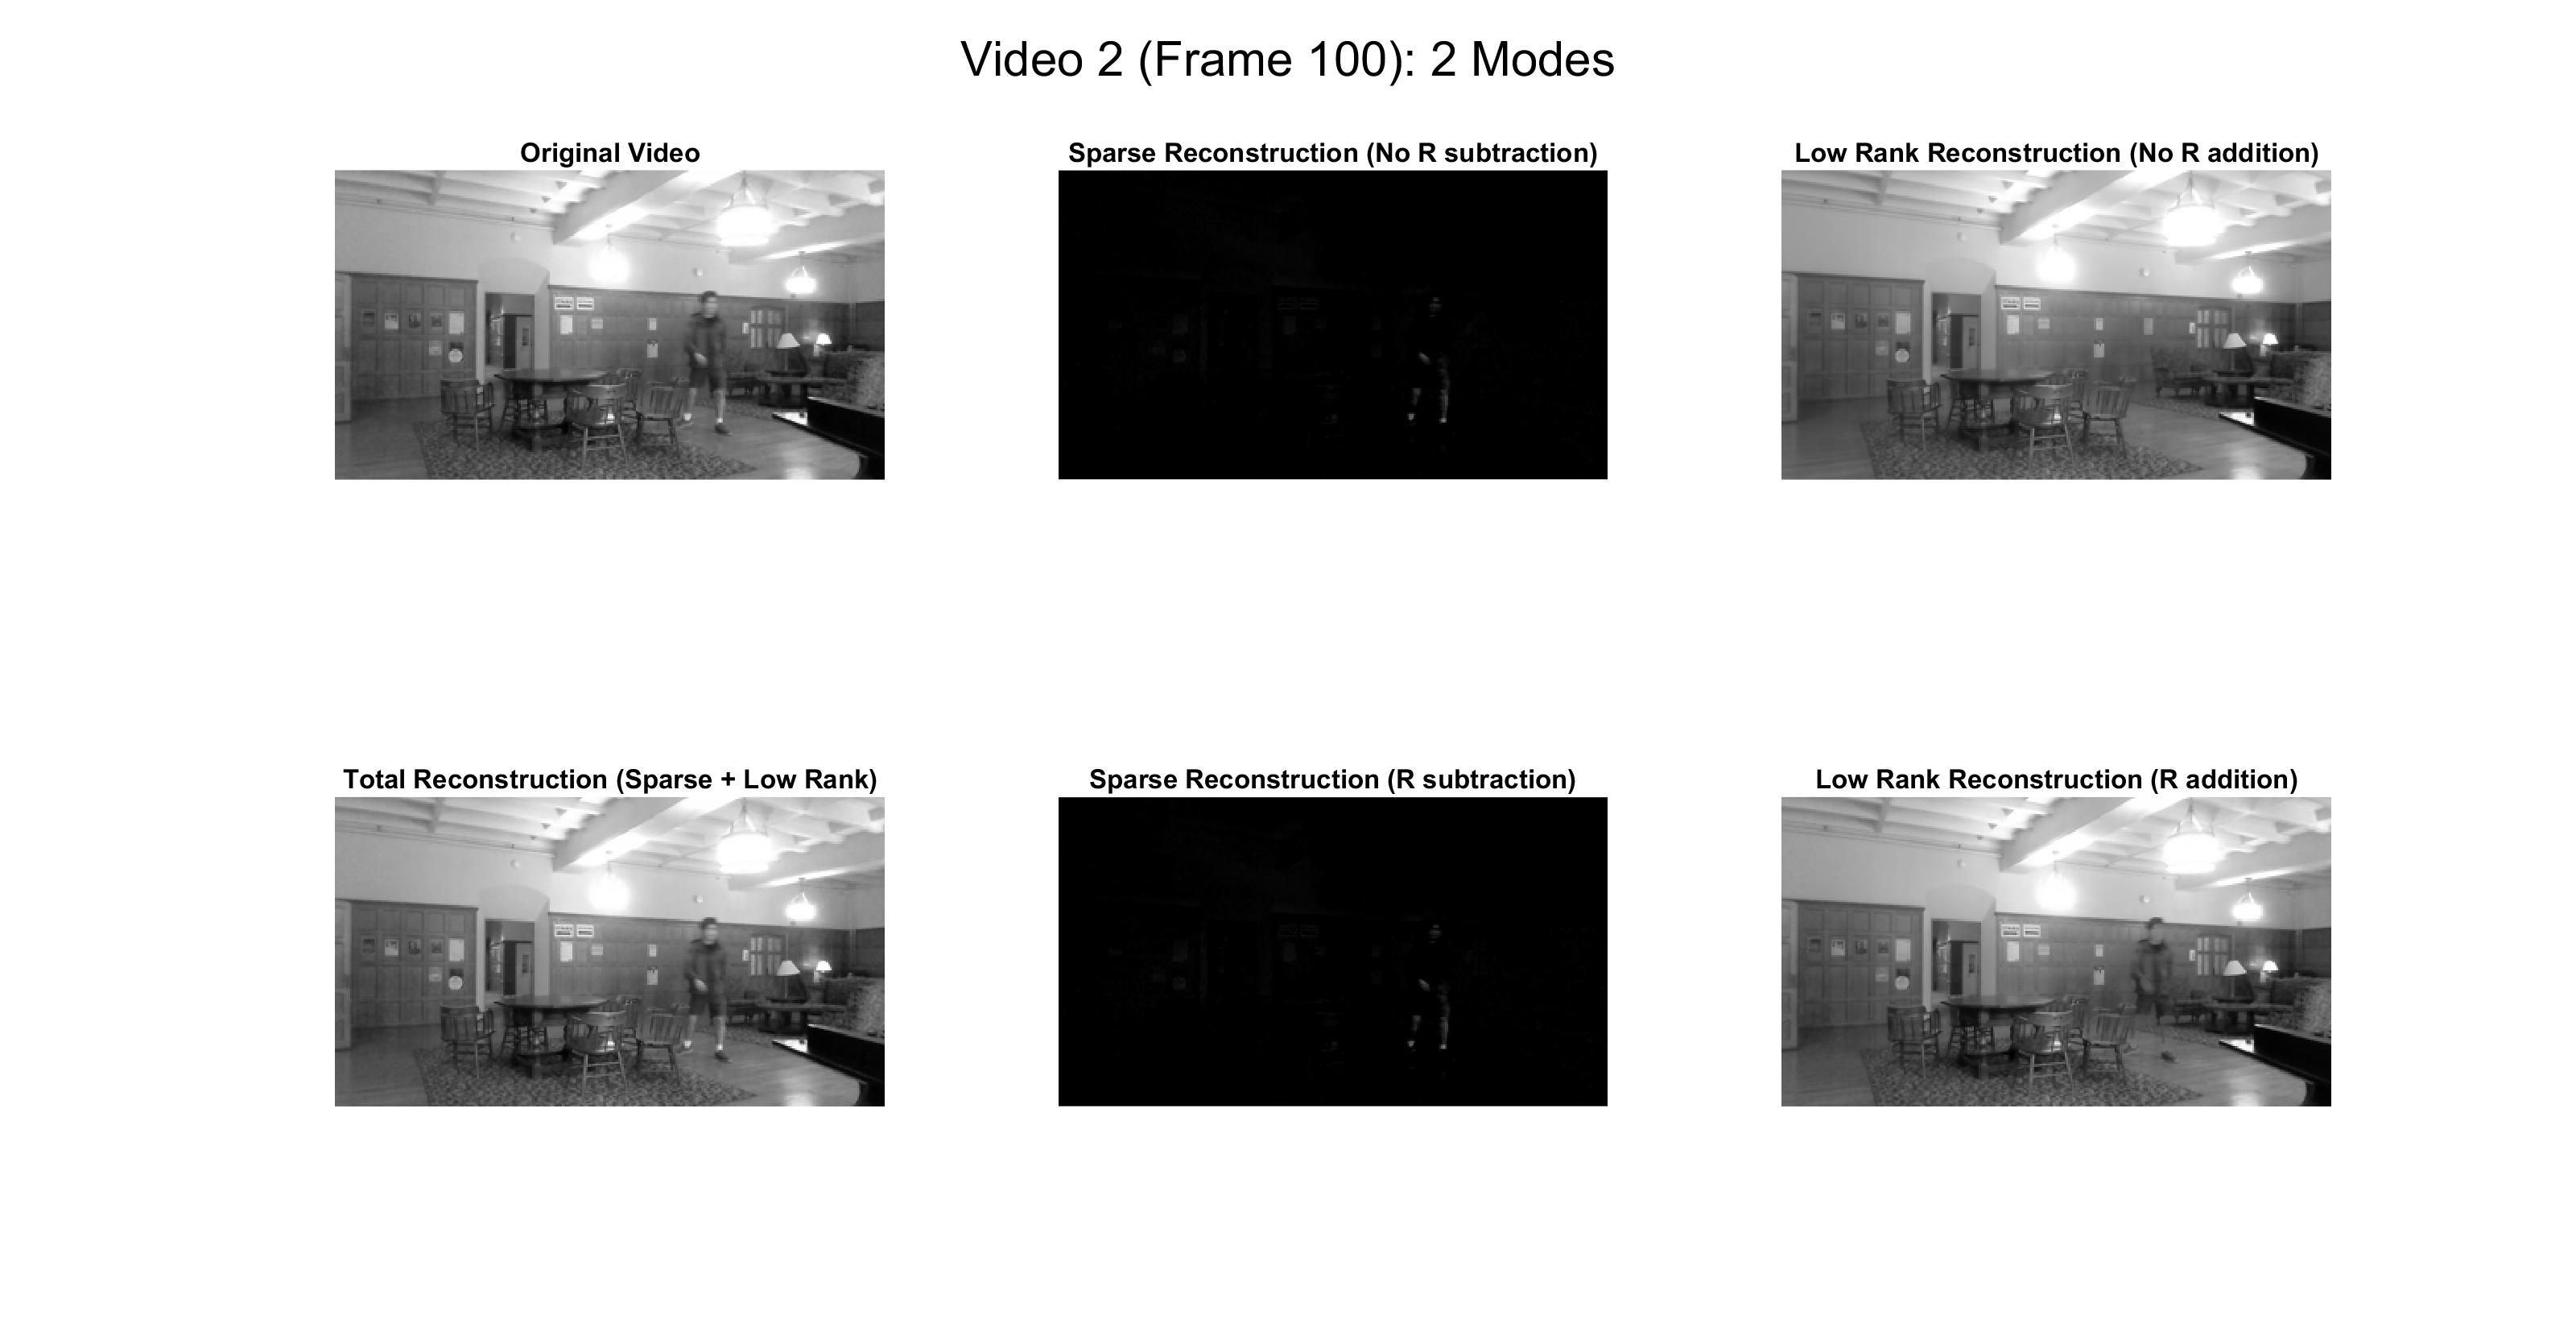
\includegraphics[width = 16cm]{vid2image}
\caption{\label{fig:scaled_diss} Video separation and reconstruction (Video 2)}
\end{center}
\end{figure}
\textbf{Video 2: Long Distance} \\
In this video, our object was still the student. The student walked around in a room (with the walls the background) at farther distances away than they did in Video 1. This was to test the effect of increasing distance - Would the student become part of the background because motion is harder to perceive farther away? \\ \\
We see that our singular value energy spectrum (Figure 3) shows that there were two dominant modes that accounted for a large portion of the energy in the system, so once again we set our "r" to this value and truncated accordingly. When we plotted our "omega" values, we saw that once again only one was very low - which showed that we realistically only needed one mode to create the background approximation using DMD (even though we used two here). \\ \\
In terms of accuracy of our DMD reconstructions, once again, the two sparse reconstructions did about the same at extracting the object. In this case, the foreground student object is a little more faint, but the sparse reconstruction did a good job of avoiding to pick up background. We see 
that once again the low-rank reconstruction without using "R" created a better background image than did the low-rank approximation that used "R". Once again, there is a small trace of the foreground image in the low-rank reconstruction that has "R" addition. Finally, our total reconstruction looks accurate again.
\begin{figure}[H]
\begin{center}
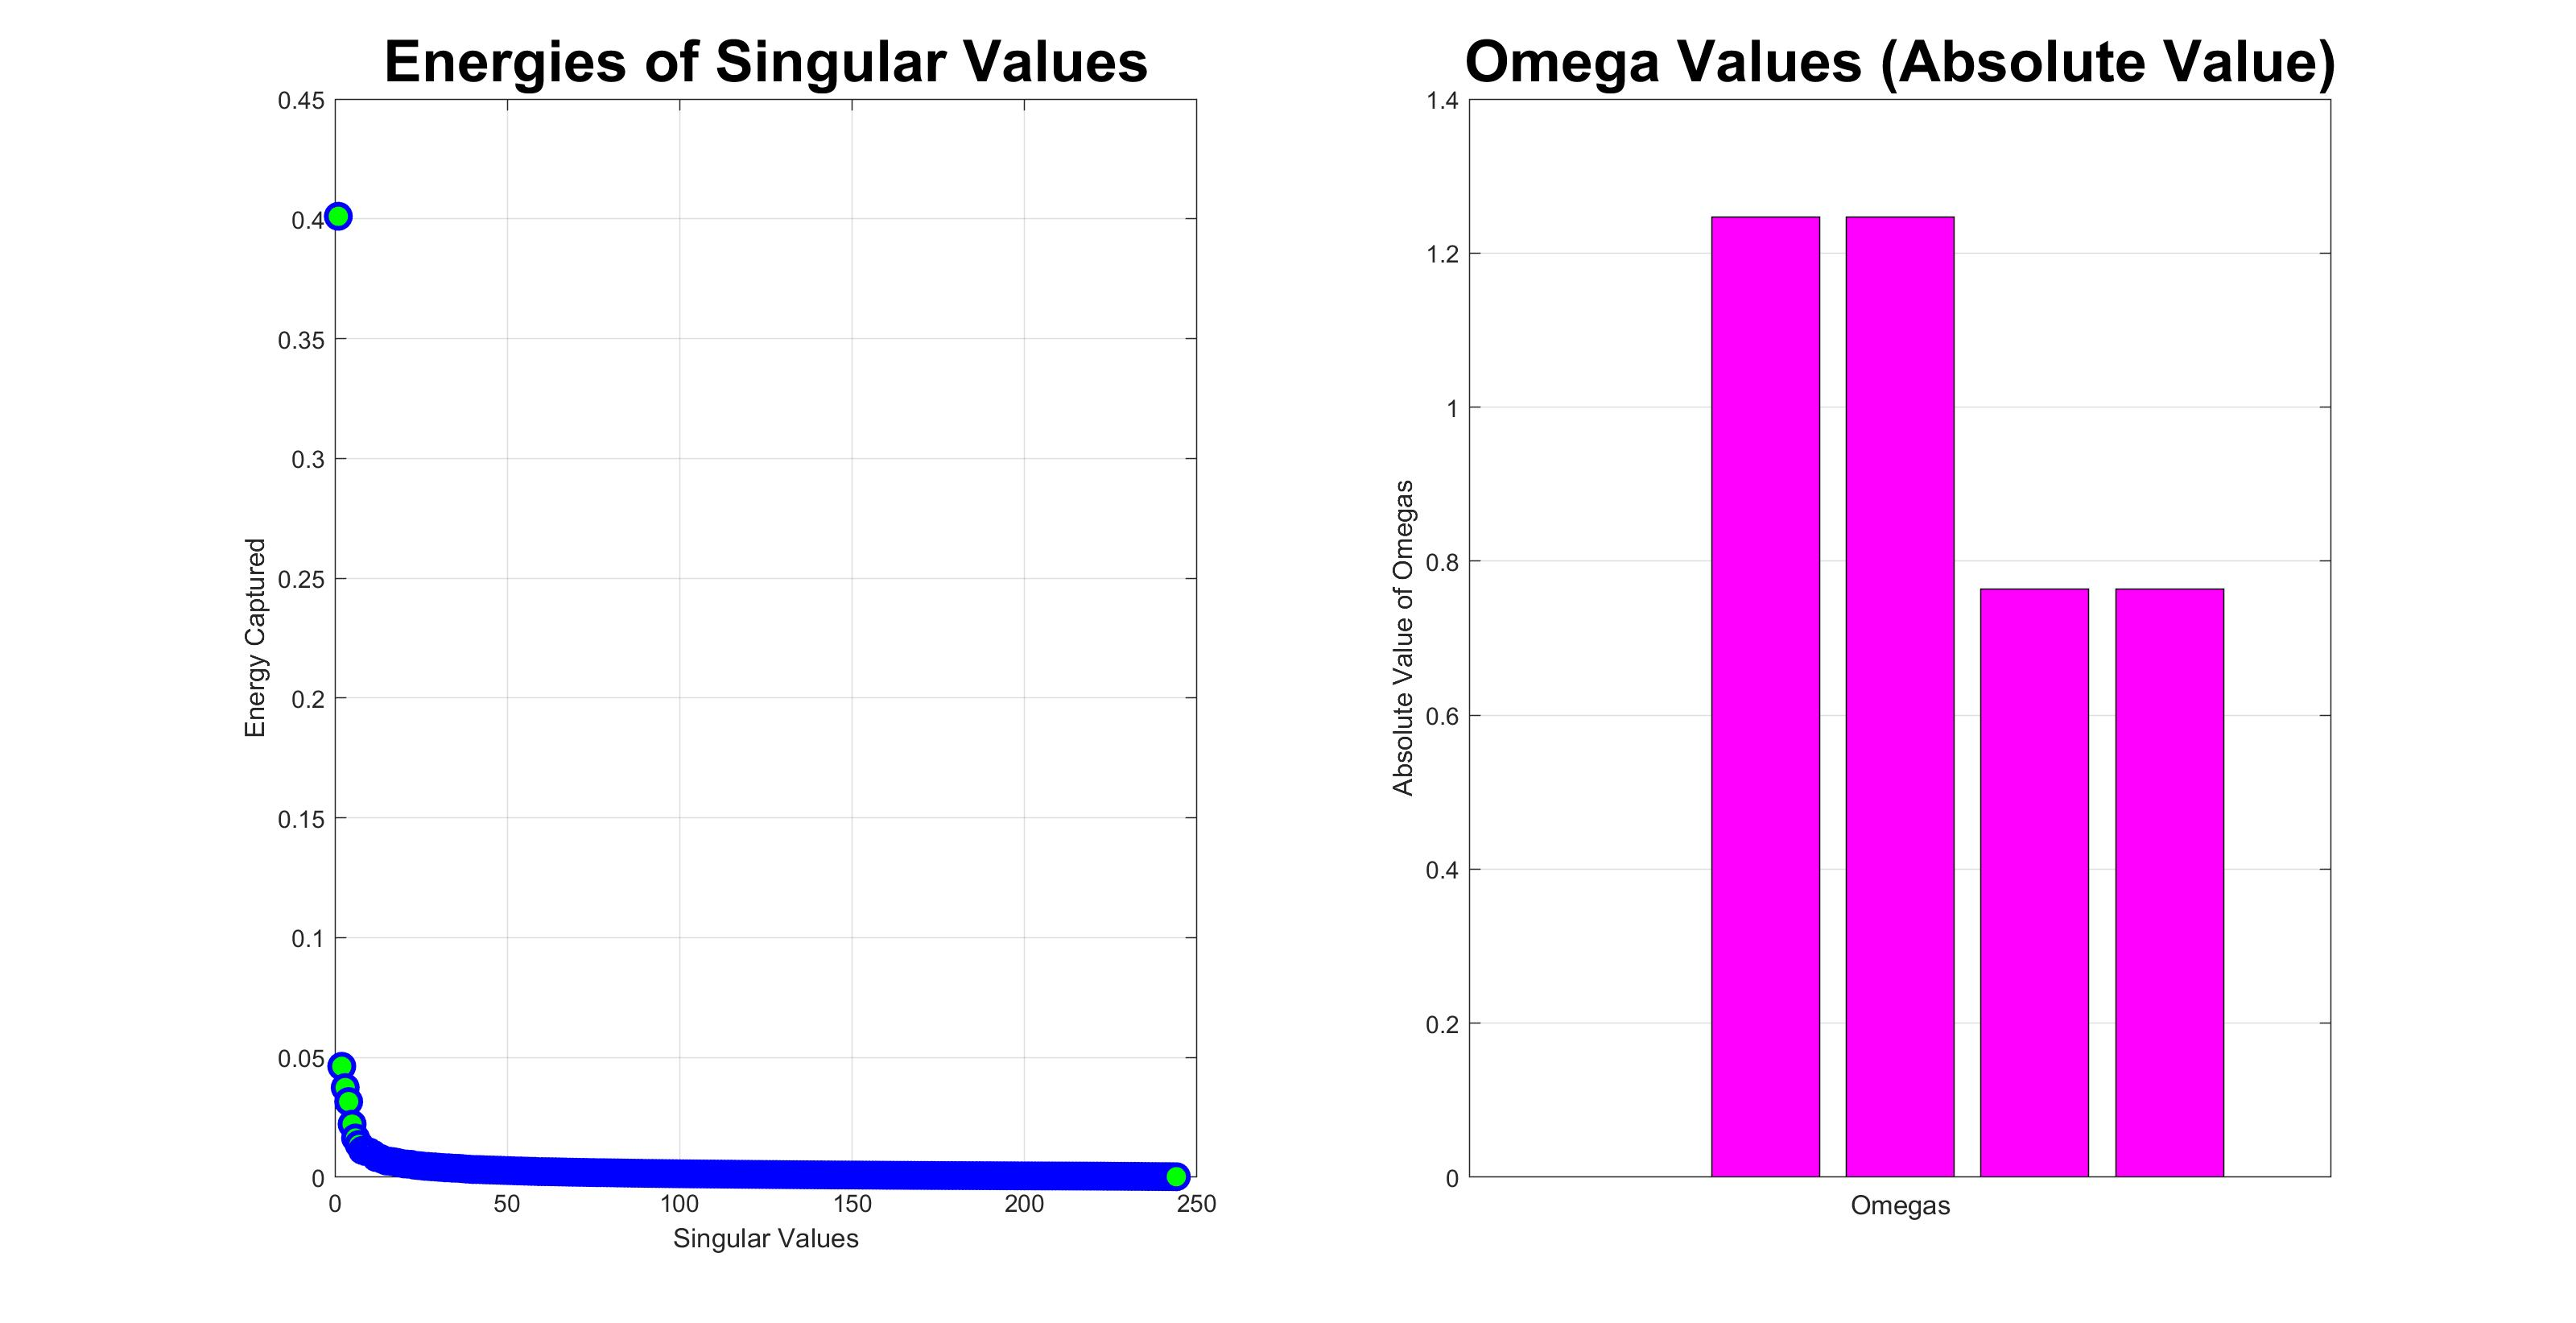
\includegraphics[width = 12cm]{energy3}
\caption{\label{fig:scaled_diss} Plots of (normalized) energy captured by singular values (left) and omega values (right) (Video 3)}
\end{center}
\end{figure}
\begin{figure}[H]
\begin{center}
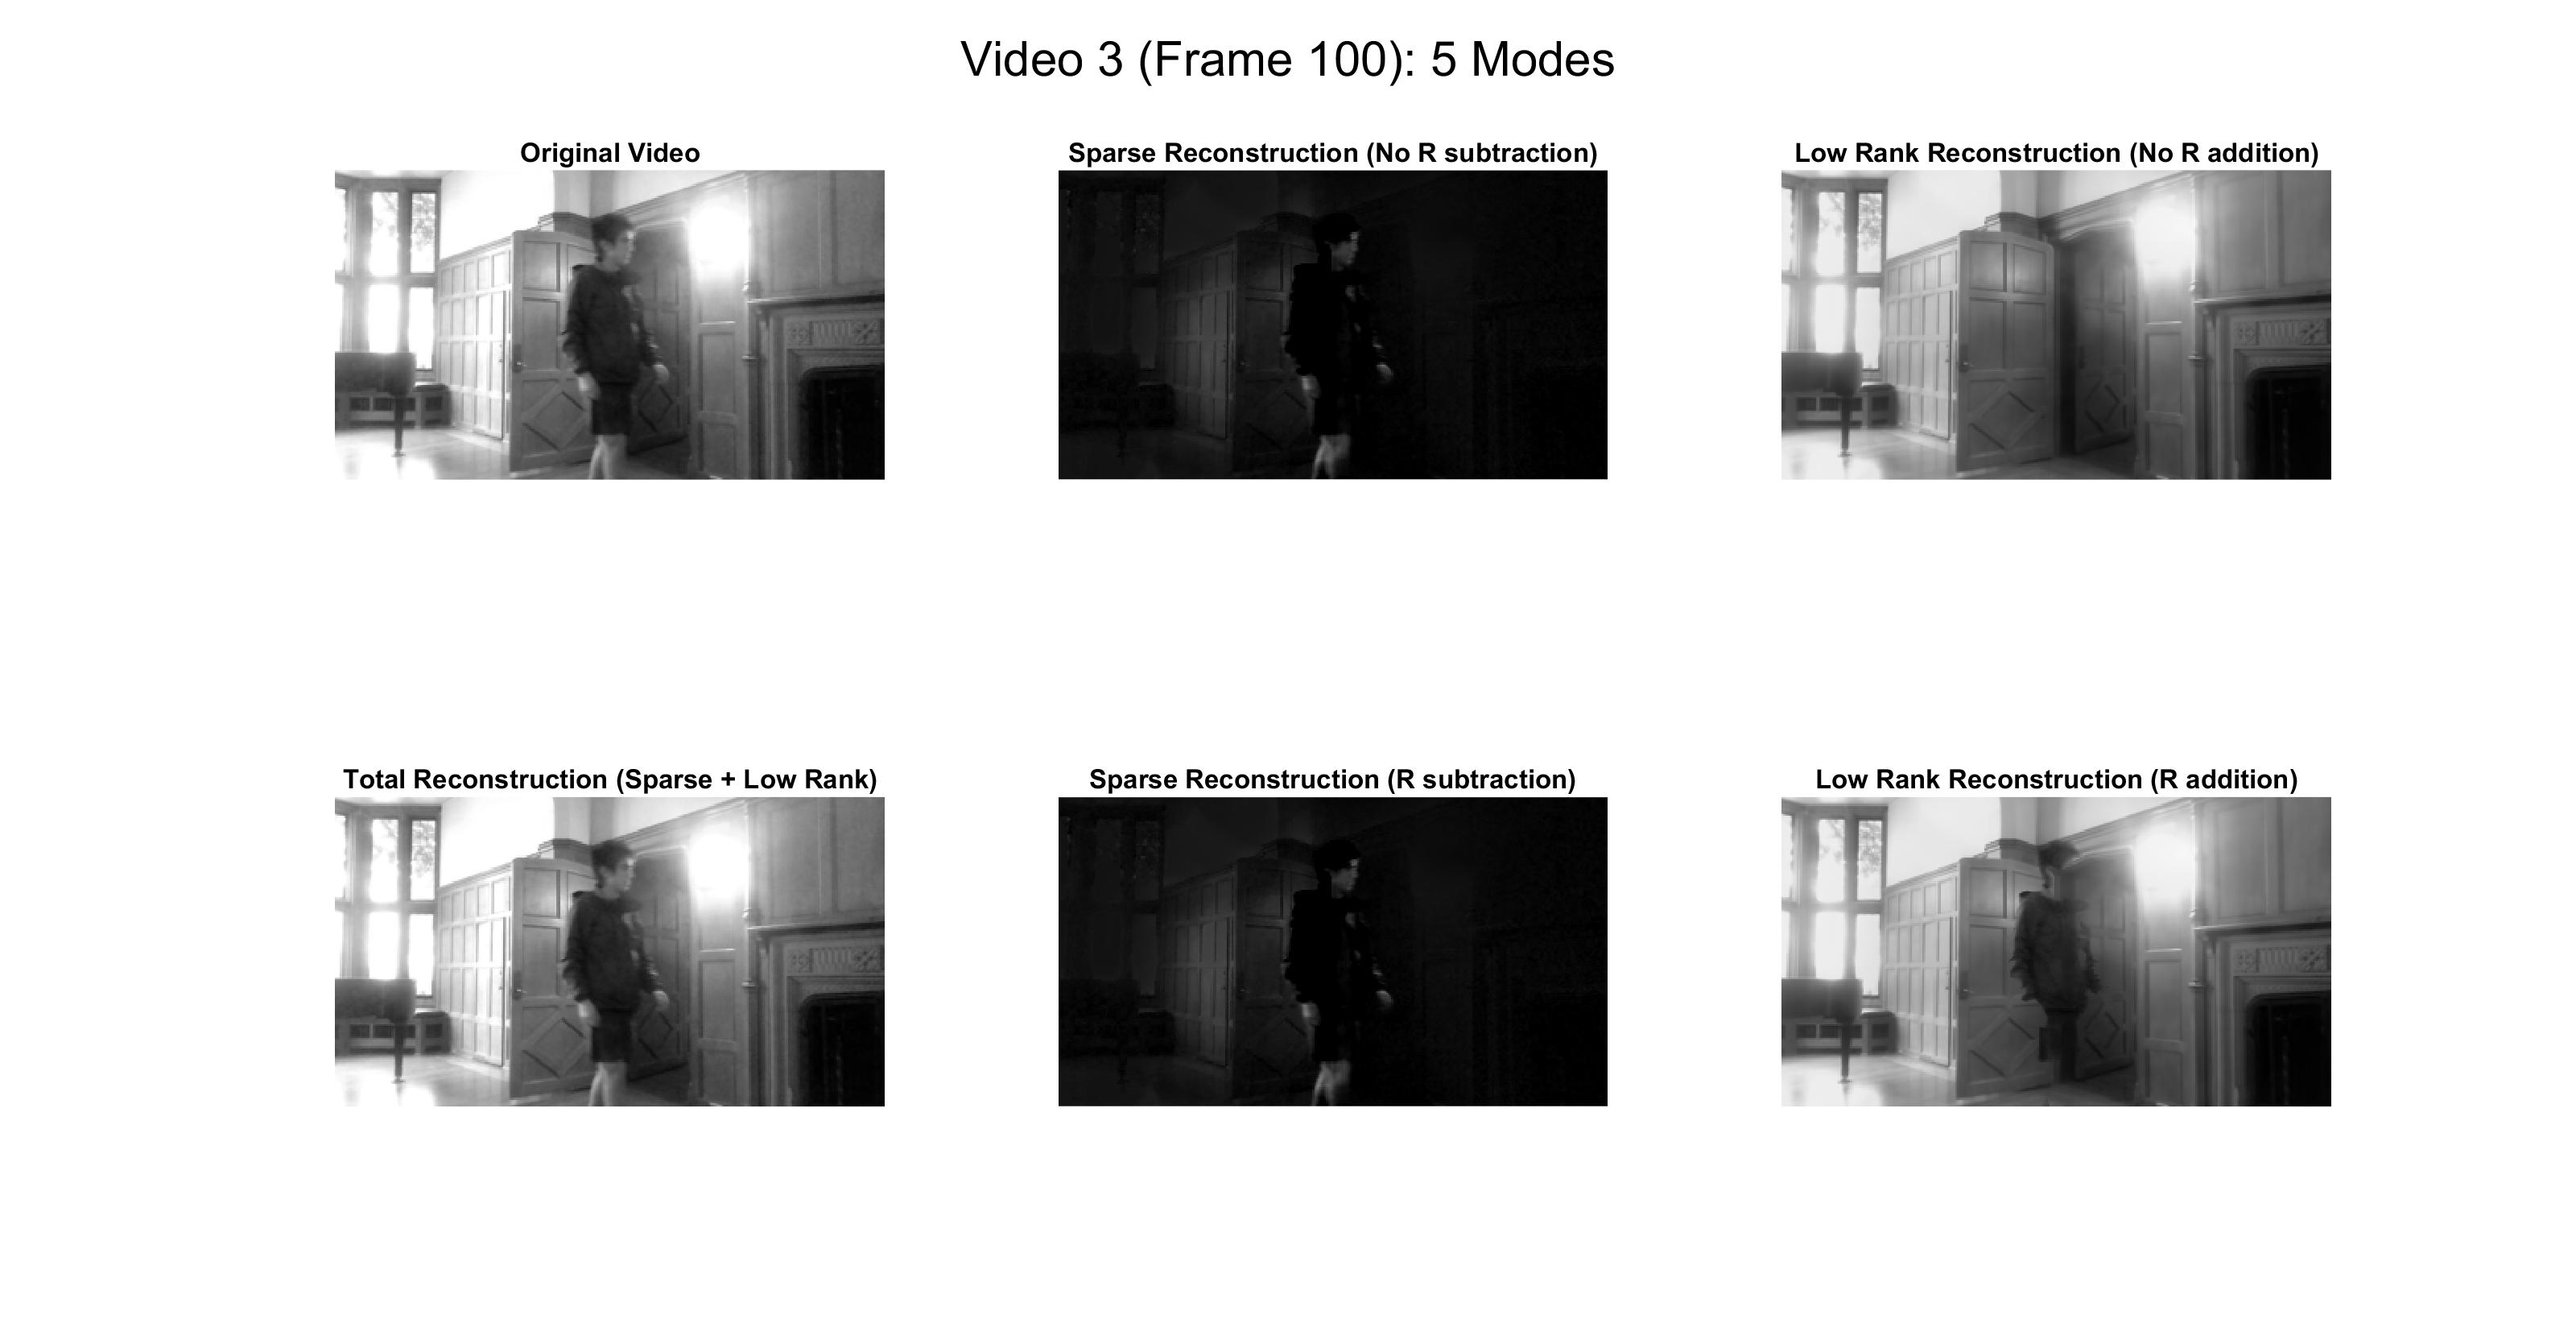
\includegraphics[width = 16cm]{vid3image}
\caption{\label{fig:scaled_diss} Video separation and reconstruction (Video 3)}
\end{center}
\end{figure}
\textbf{Video 3: Brighter Background} \\
In this video, we changed the scenario by increasing the brightness of the background to increase visual separation between the foreground and background object. We achieved this by filming towards a light and a window, both of which contributed light. Our foreground object was the same distance relatively as in Video 1 (ideal case). \\ \\
We see via Figure 5 that our energy captured by the singular values makes it harder to distinguish how many modes truly can represent this system, since it goes down like a gradient. However, we chose to use 5 modes for this video as the first 5 modes all captured somewhat significant portions of the energy of the system. The plot of omega values shows how small the first omega is - It is so low that it cannot be visualized on the graph at the same scale that the other four omega values are at! Once again, it seems that we could have done this reconstruction with only one mode instead of five. \\ \\
We see from our reconstructions that the sparse reconstruction in both cases does a good job of clearly showing the moving foreground object, although it does pick up a little bit of the background (to the left). Once again, the low-rank reconstruction without R addition does a great job of showing the background, while the low-rank reconstruction with R addition had trace remnants of the object. Finally, the total reconstruction is good once again.

\begin{figure}[H]
\begin{center}
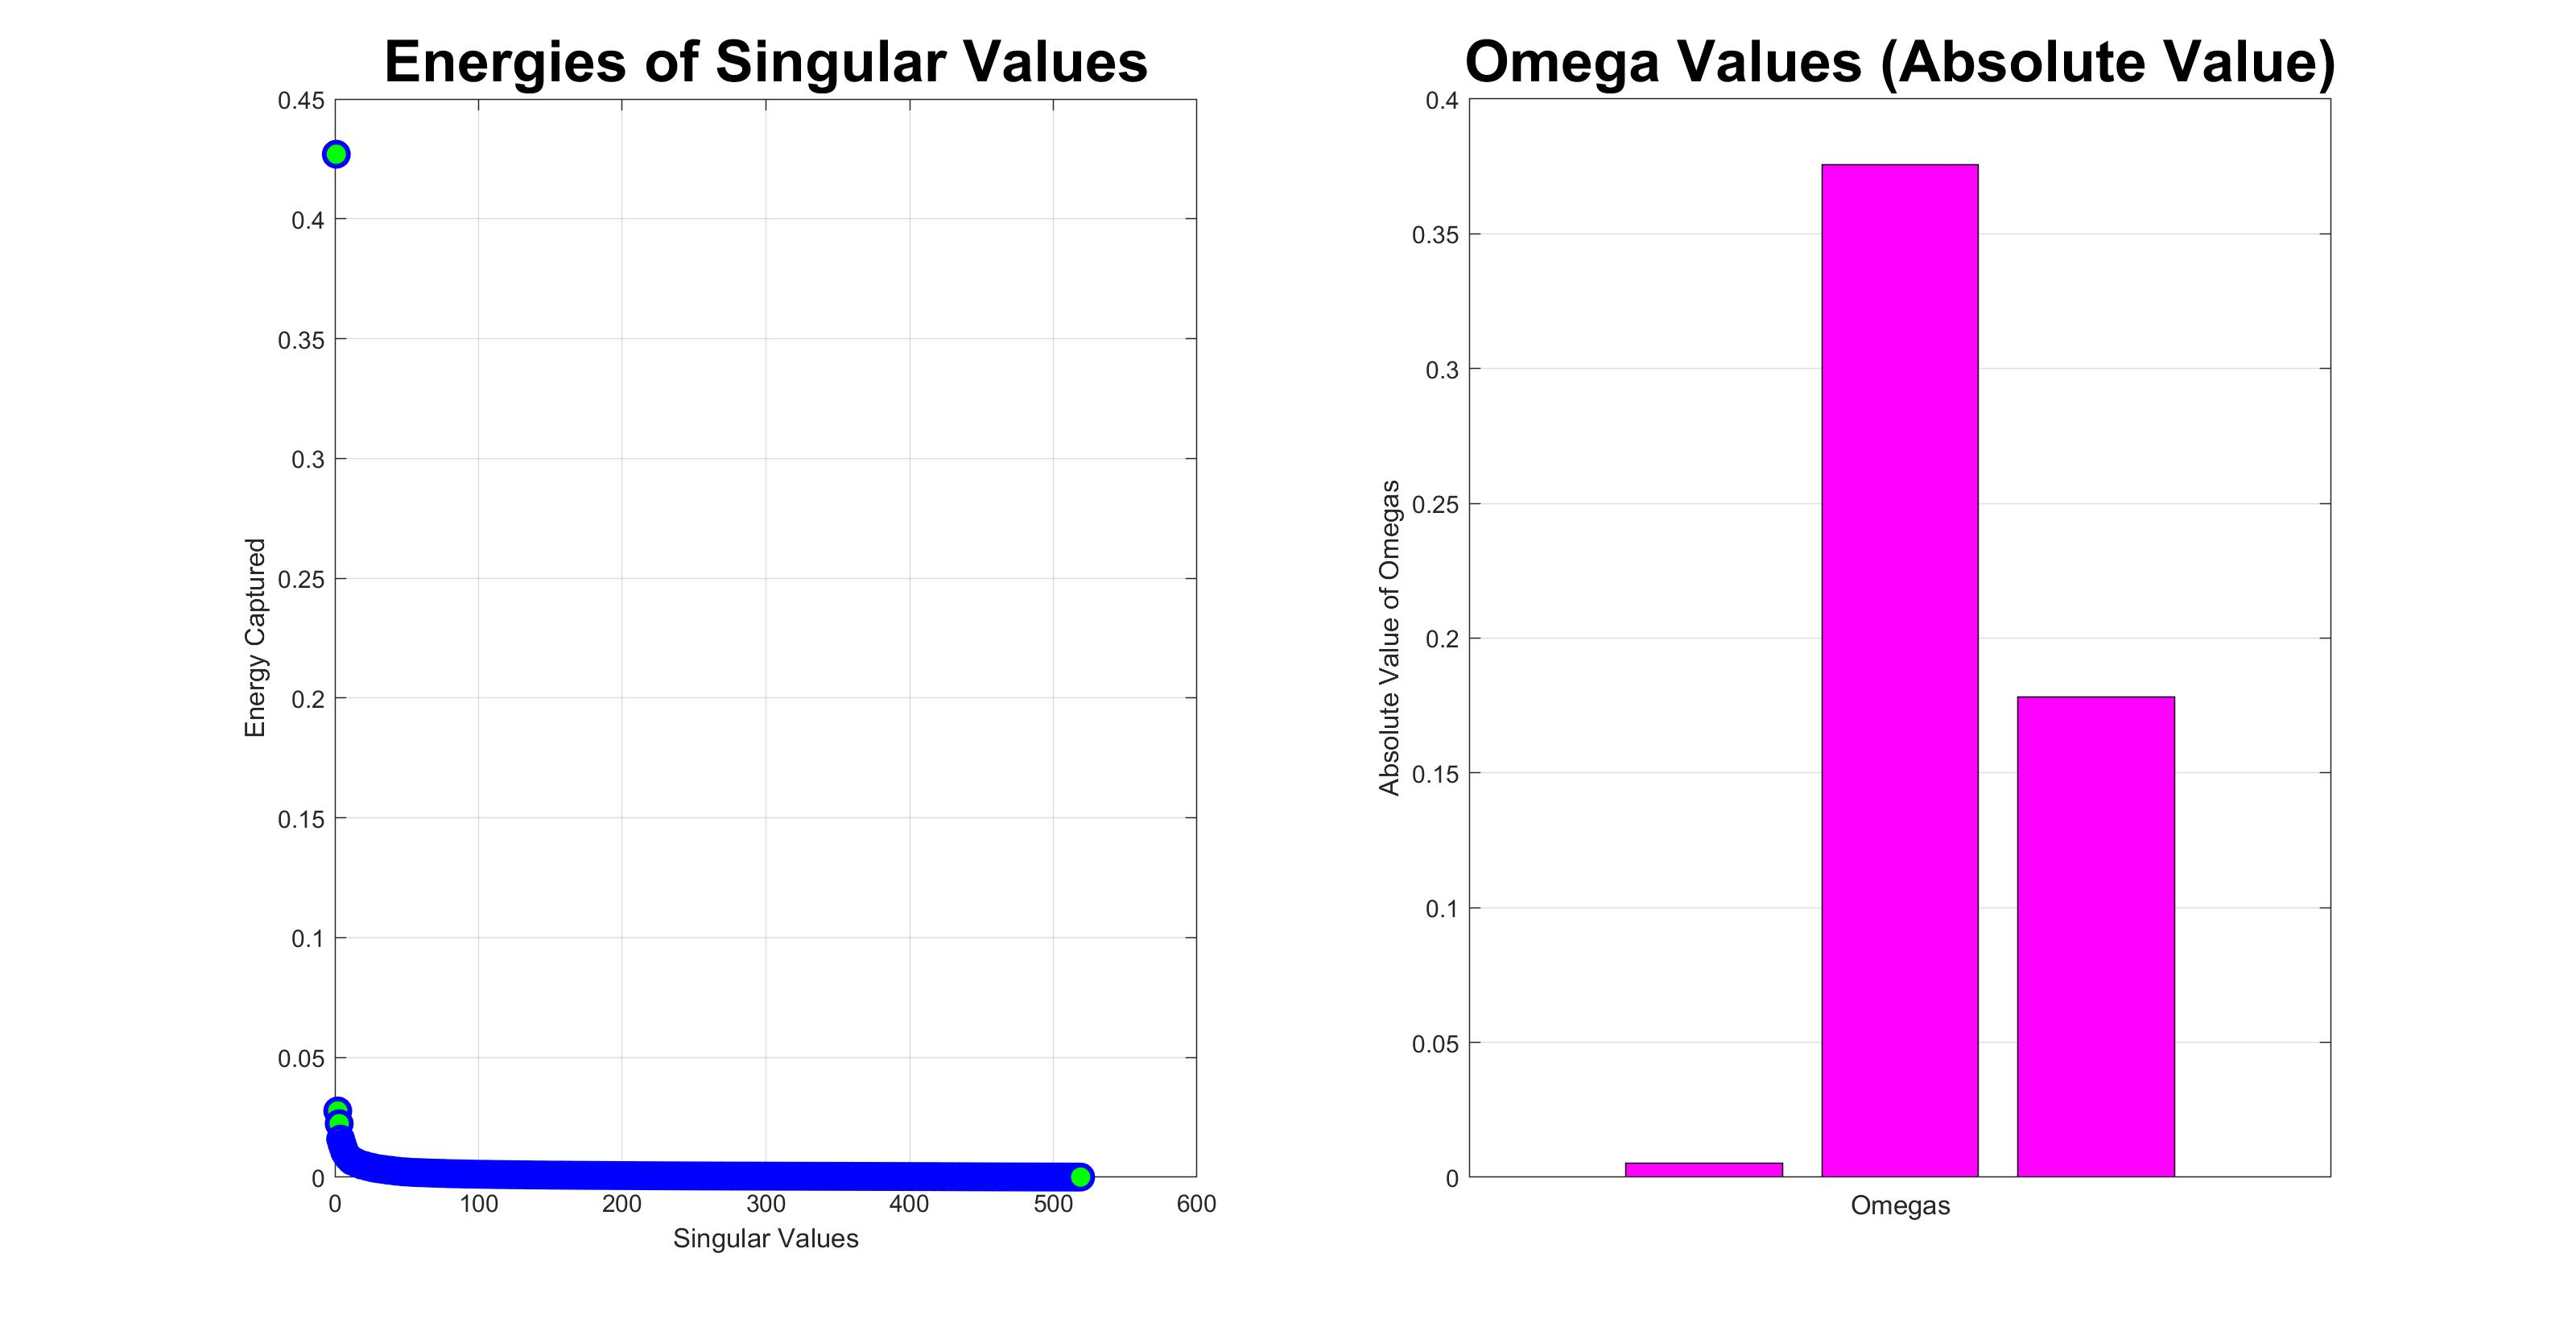
\includegraphics[width = 12cm]{energy4}
\caption{\label{fig:scaled_diss} Plots of (normalized) energy captured by singular values (left) and omega values (right) (Video 4)}
\end{center}
\end{figure}
\begin{figure}[H]
\begin{center}
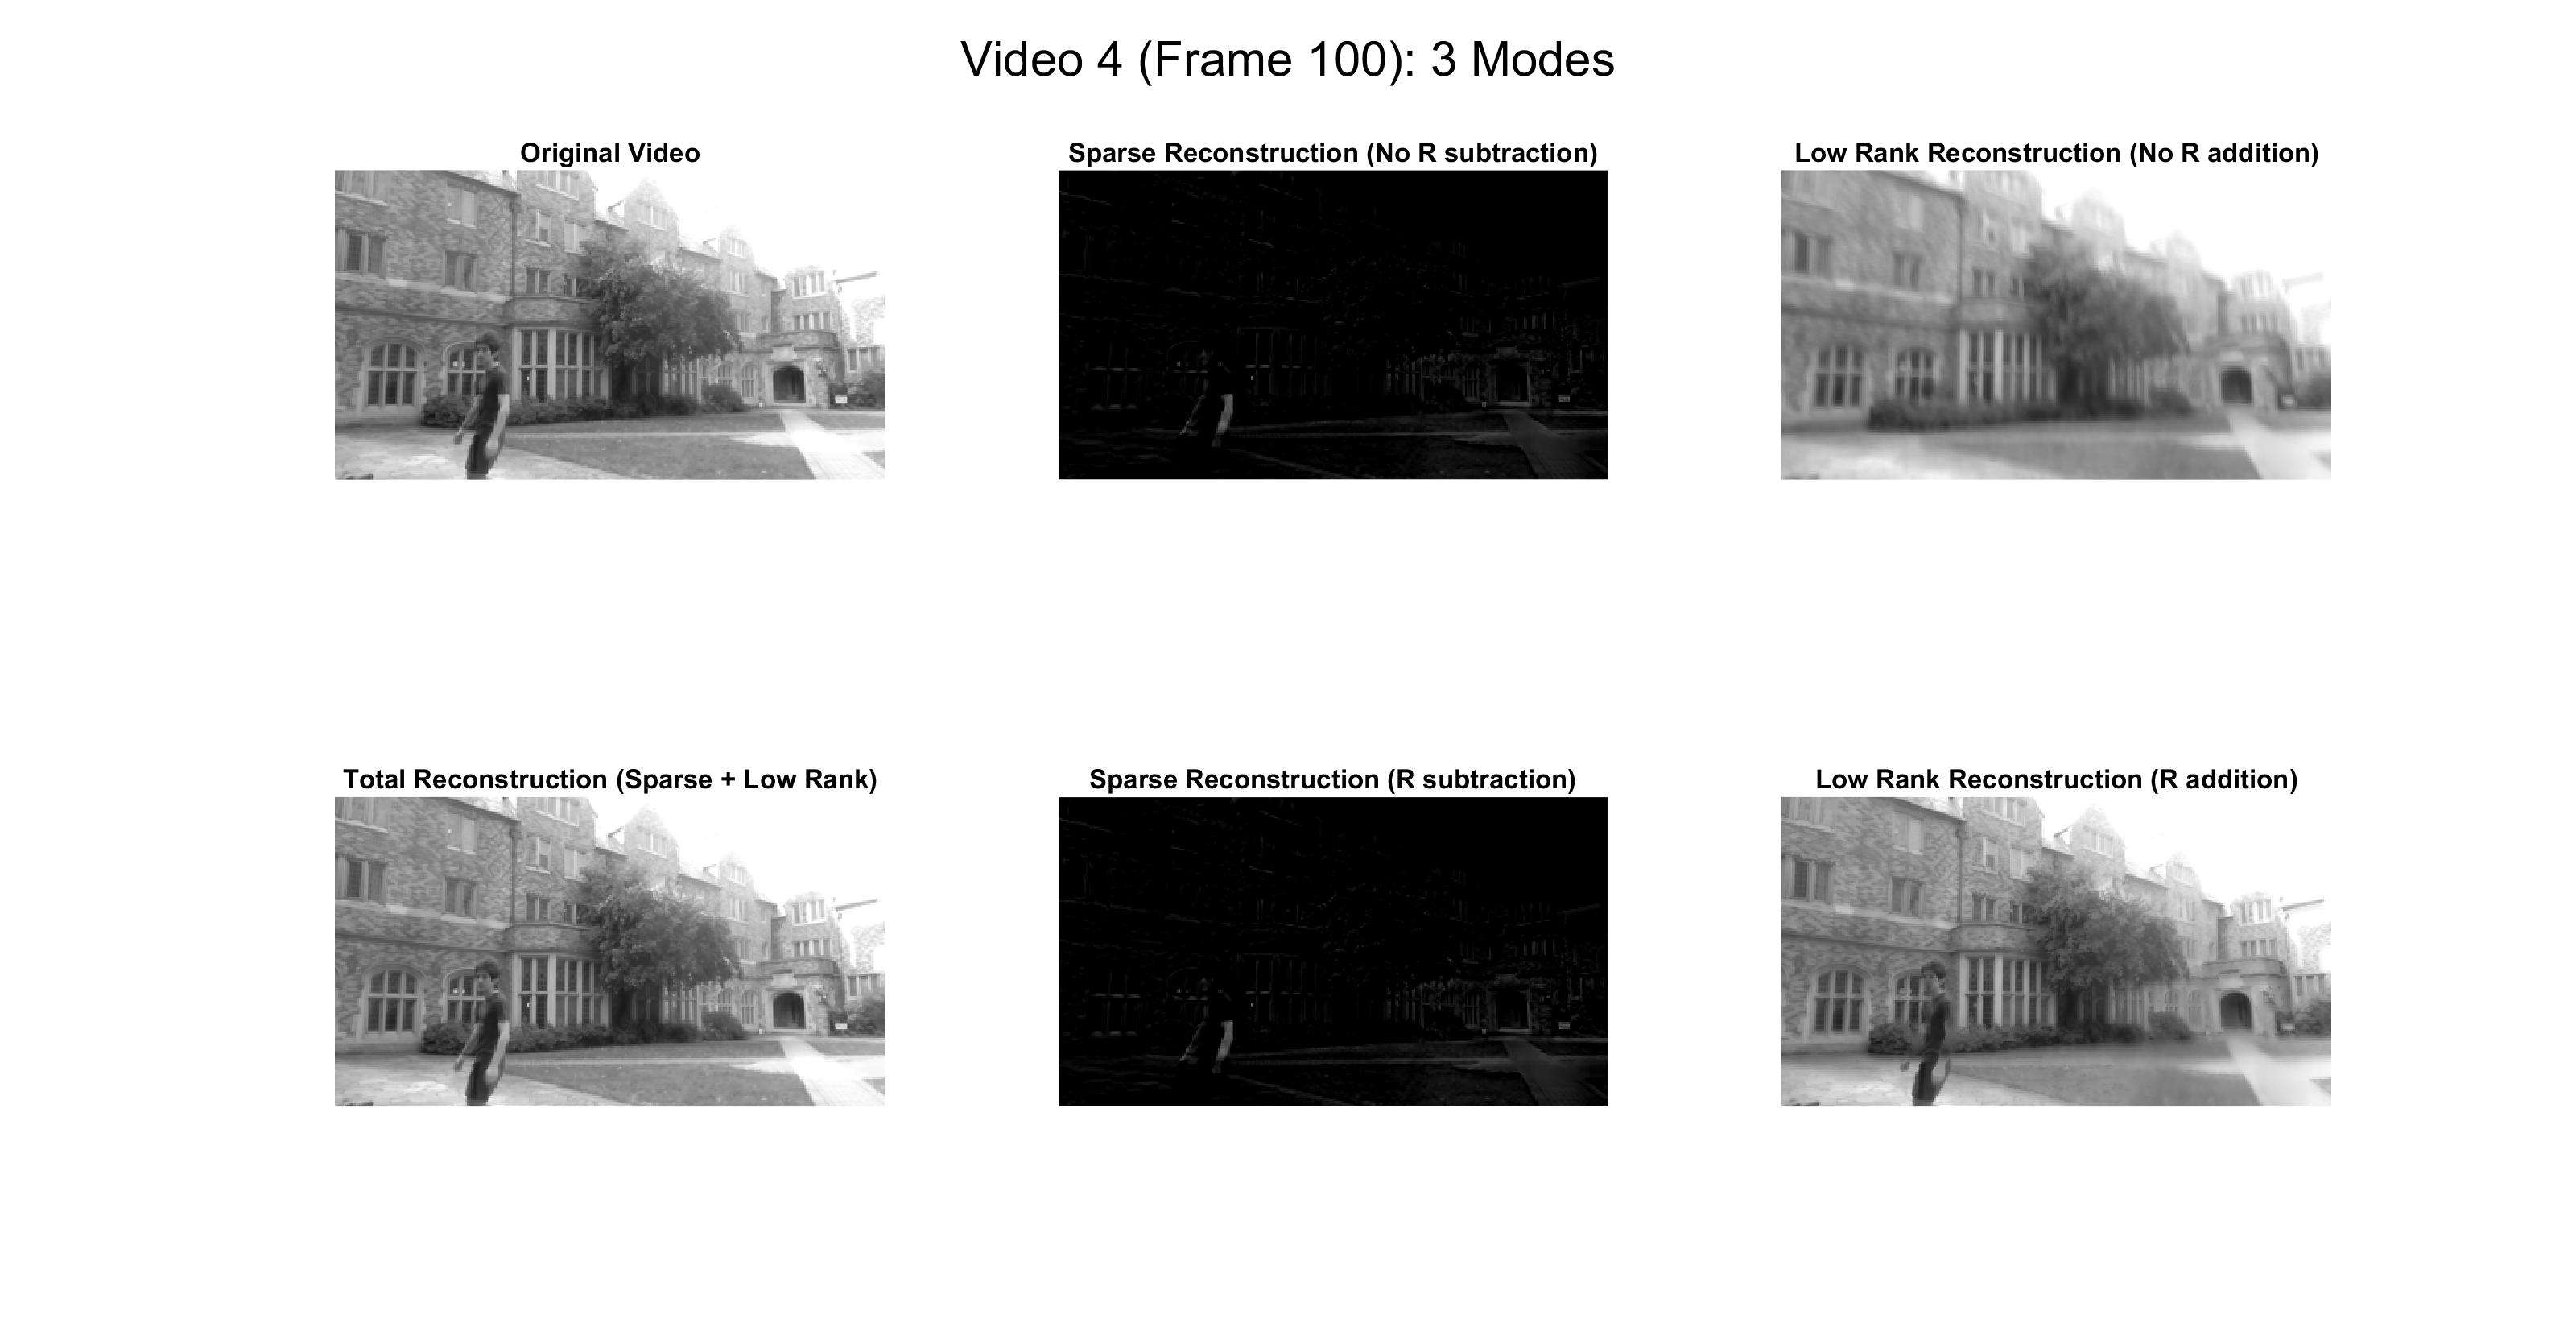
\includegraphics[width = 16cm]{vid4image}
\caption{\label{fig:scaled_diss} Video separation and reconstruction (Video 4)}
\end{center}
\end{figure}
\textbf{Video 4: Light Noise} \\ \\
In this video, we changed the scenario by adding noise to the system. Previously, the laptop was placed on a table while recording, and was therefore stationary and had virtually no noise introduced due to shaky camera. However, in this case, we had a person hold the laptop as still as they could. Although humans can hold things pretty steady, there will still be some slight shaking, and there will be much more noise introduced than if the recording device was sitting on a table. We introduced this light noise to see what it's effects on the reconstruction were. \\ \\
From our singular value plot, we saw approximately three significant modes that we used. Once again, our plot of "omega" values showed that only one of these modes was relatively low and contributed to the background approximation. Nevertheless, we continued on with three modes. \\ \\
We see that even with a slight amount of noise introduced, both sparse reconstructions do not pick up the foreground object as well as they did in the previous three scenarios. Both sparse reconstructions show only slight traces of the object, and pick up some of the background to the right. Although both of the sparse reconstructions are similar, we do see major differences in the low-rank reconstructions. In terms of the low-rank reconstruction without "R" addition, we see that the background looks blurry, which is probably a result of the slight noise introduced; however, we see that there is still a complete removal of the foreground object from the background. The low-rank reconstruction with "R" addition is less blurry, but does a poor job of removing the foreground object. Both the foreground and the background are both clearly visible still, so it does not do a good job. Once again, our total reconstruction matches our original video.
\begin{figure}[H]
\begin{center}
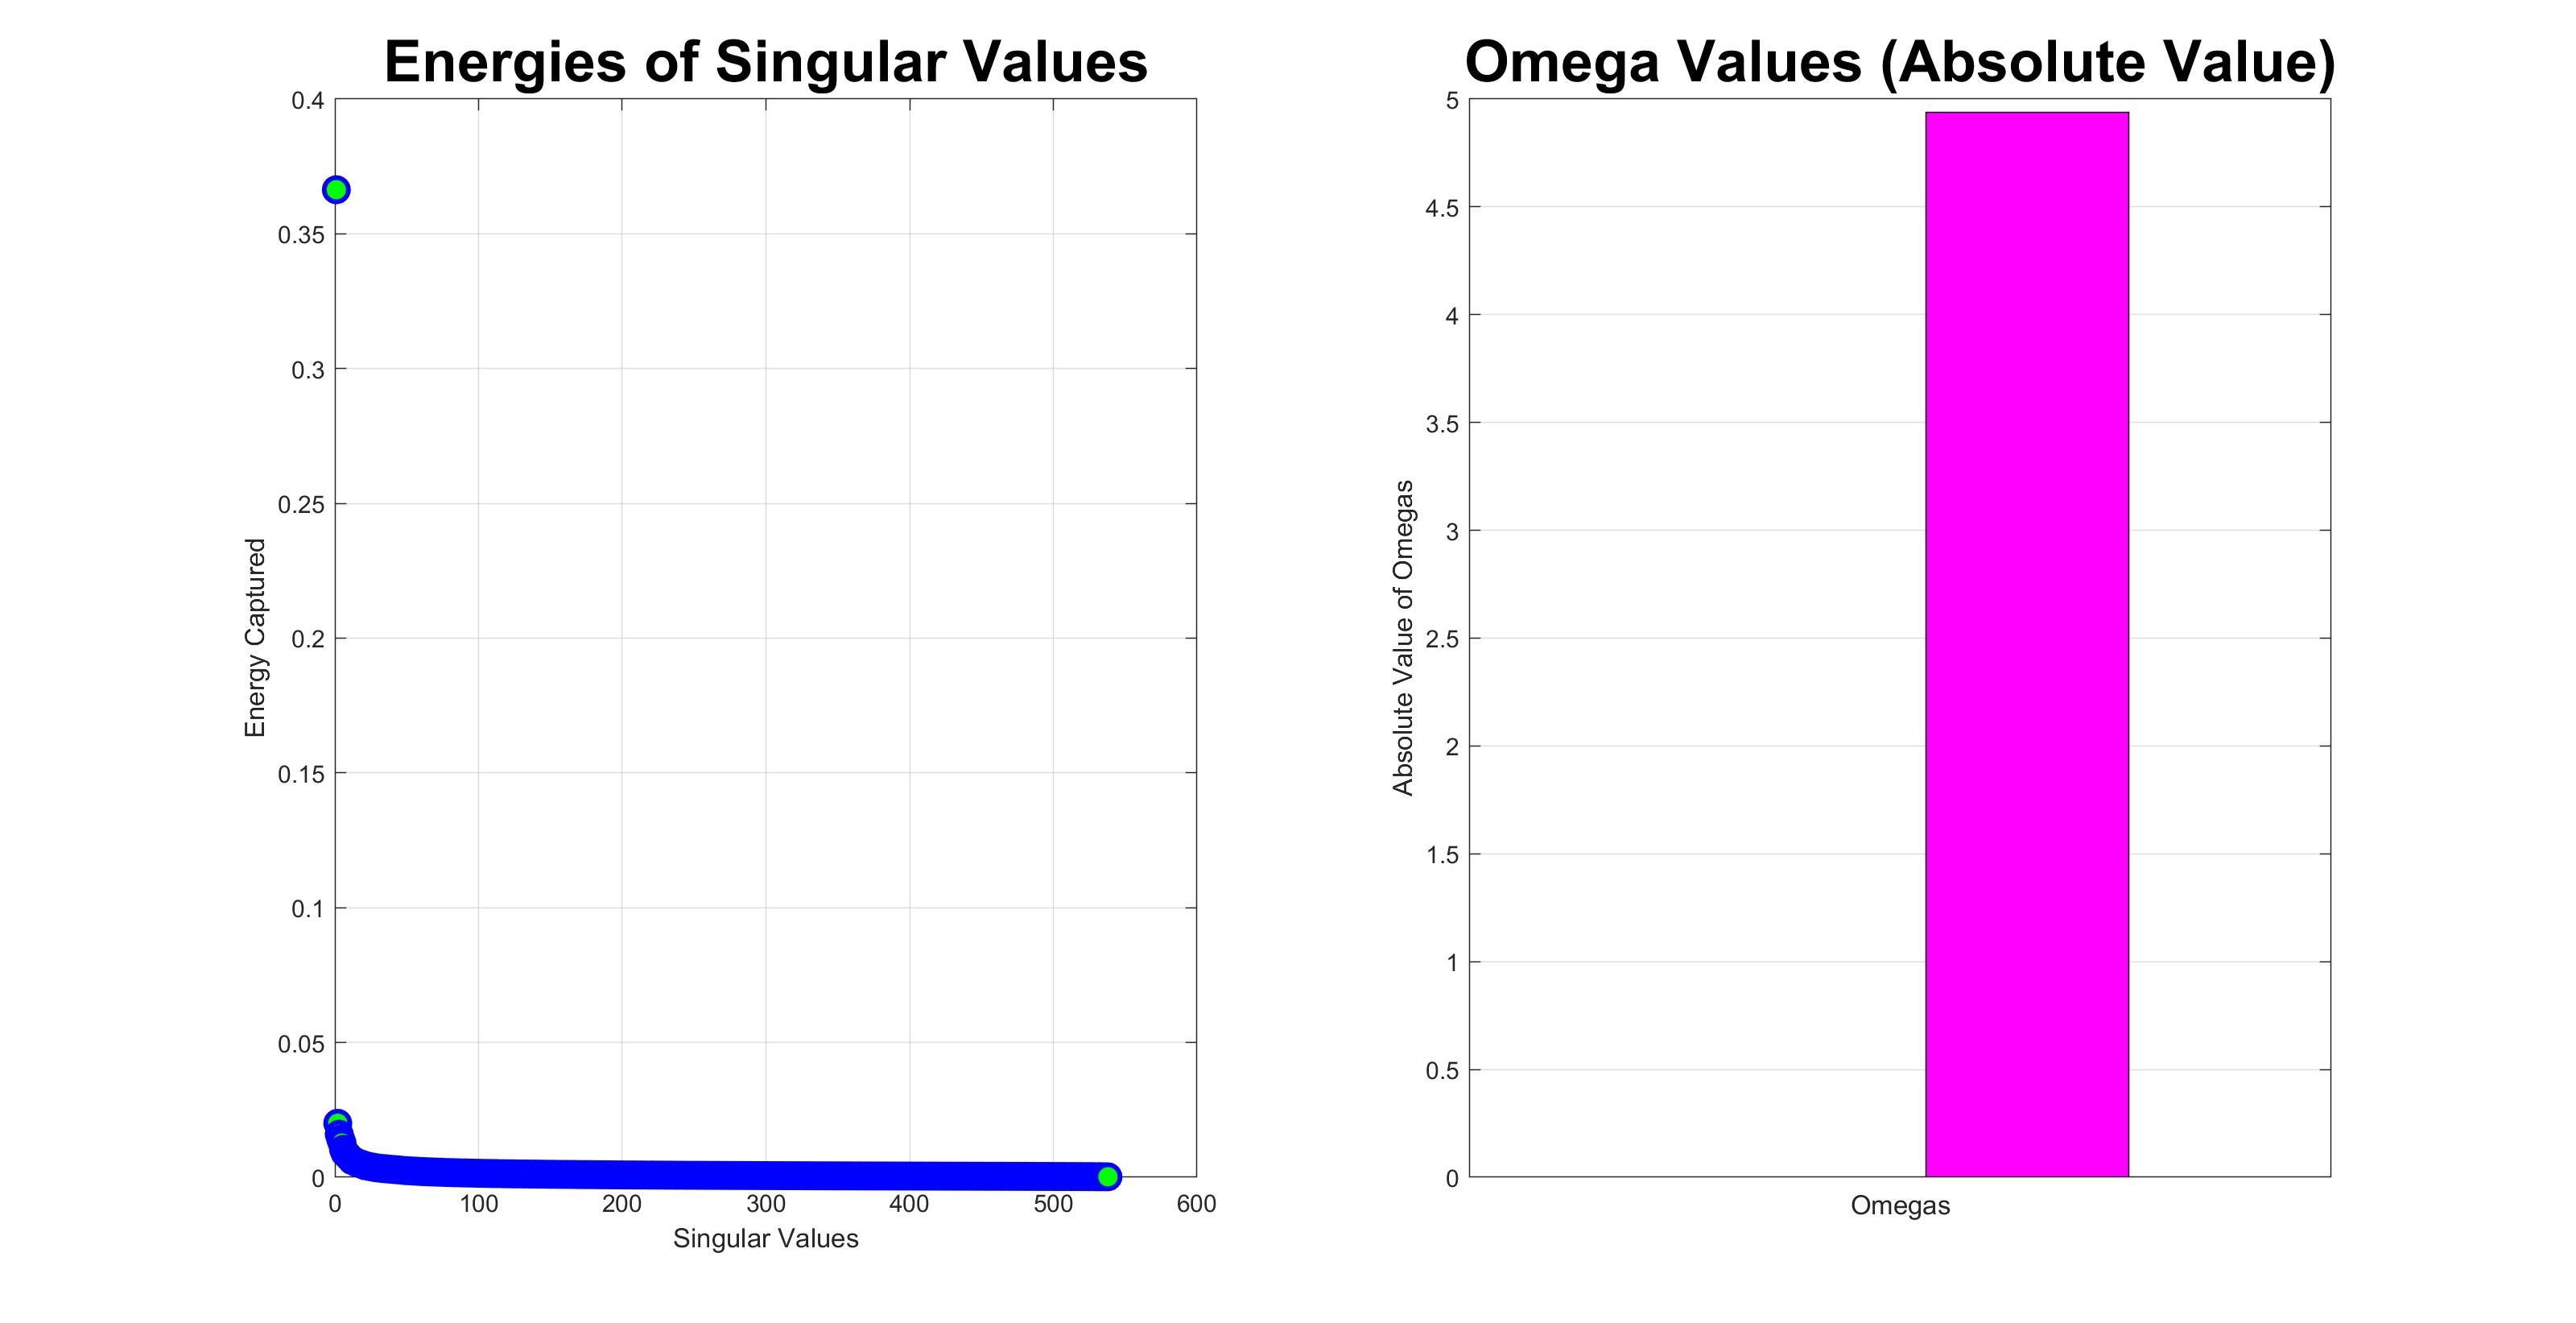
\includegraphics[width = 12cm]{energy5}
\caption{\label{fig:scaled_diss} Plots of (normalized) energy captured by singular values (left) and omega values (right) (Video 4)}
\end{center}
\end{figure}
\begin{figure}[H]
\begin{center}
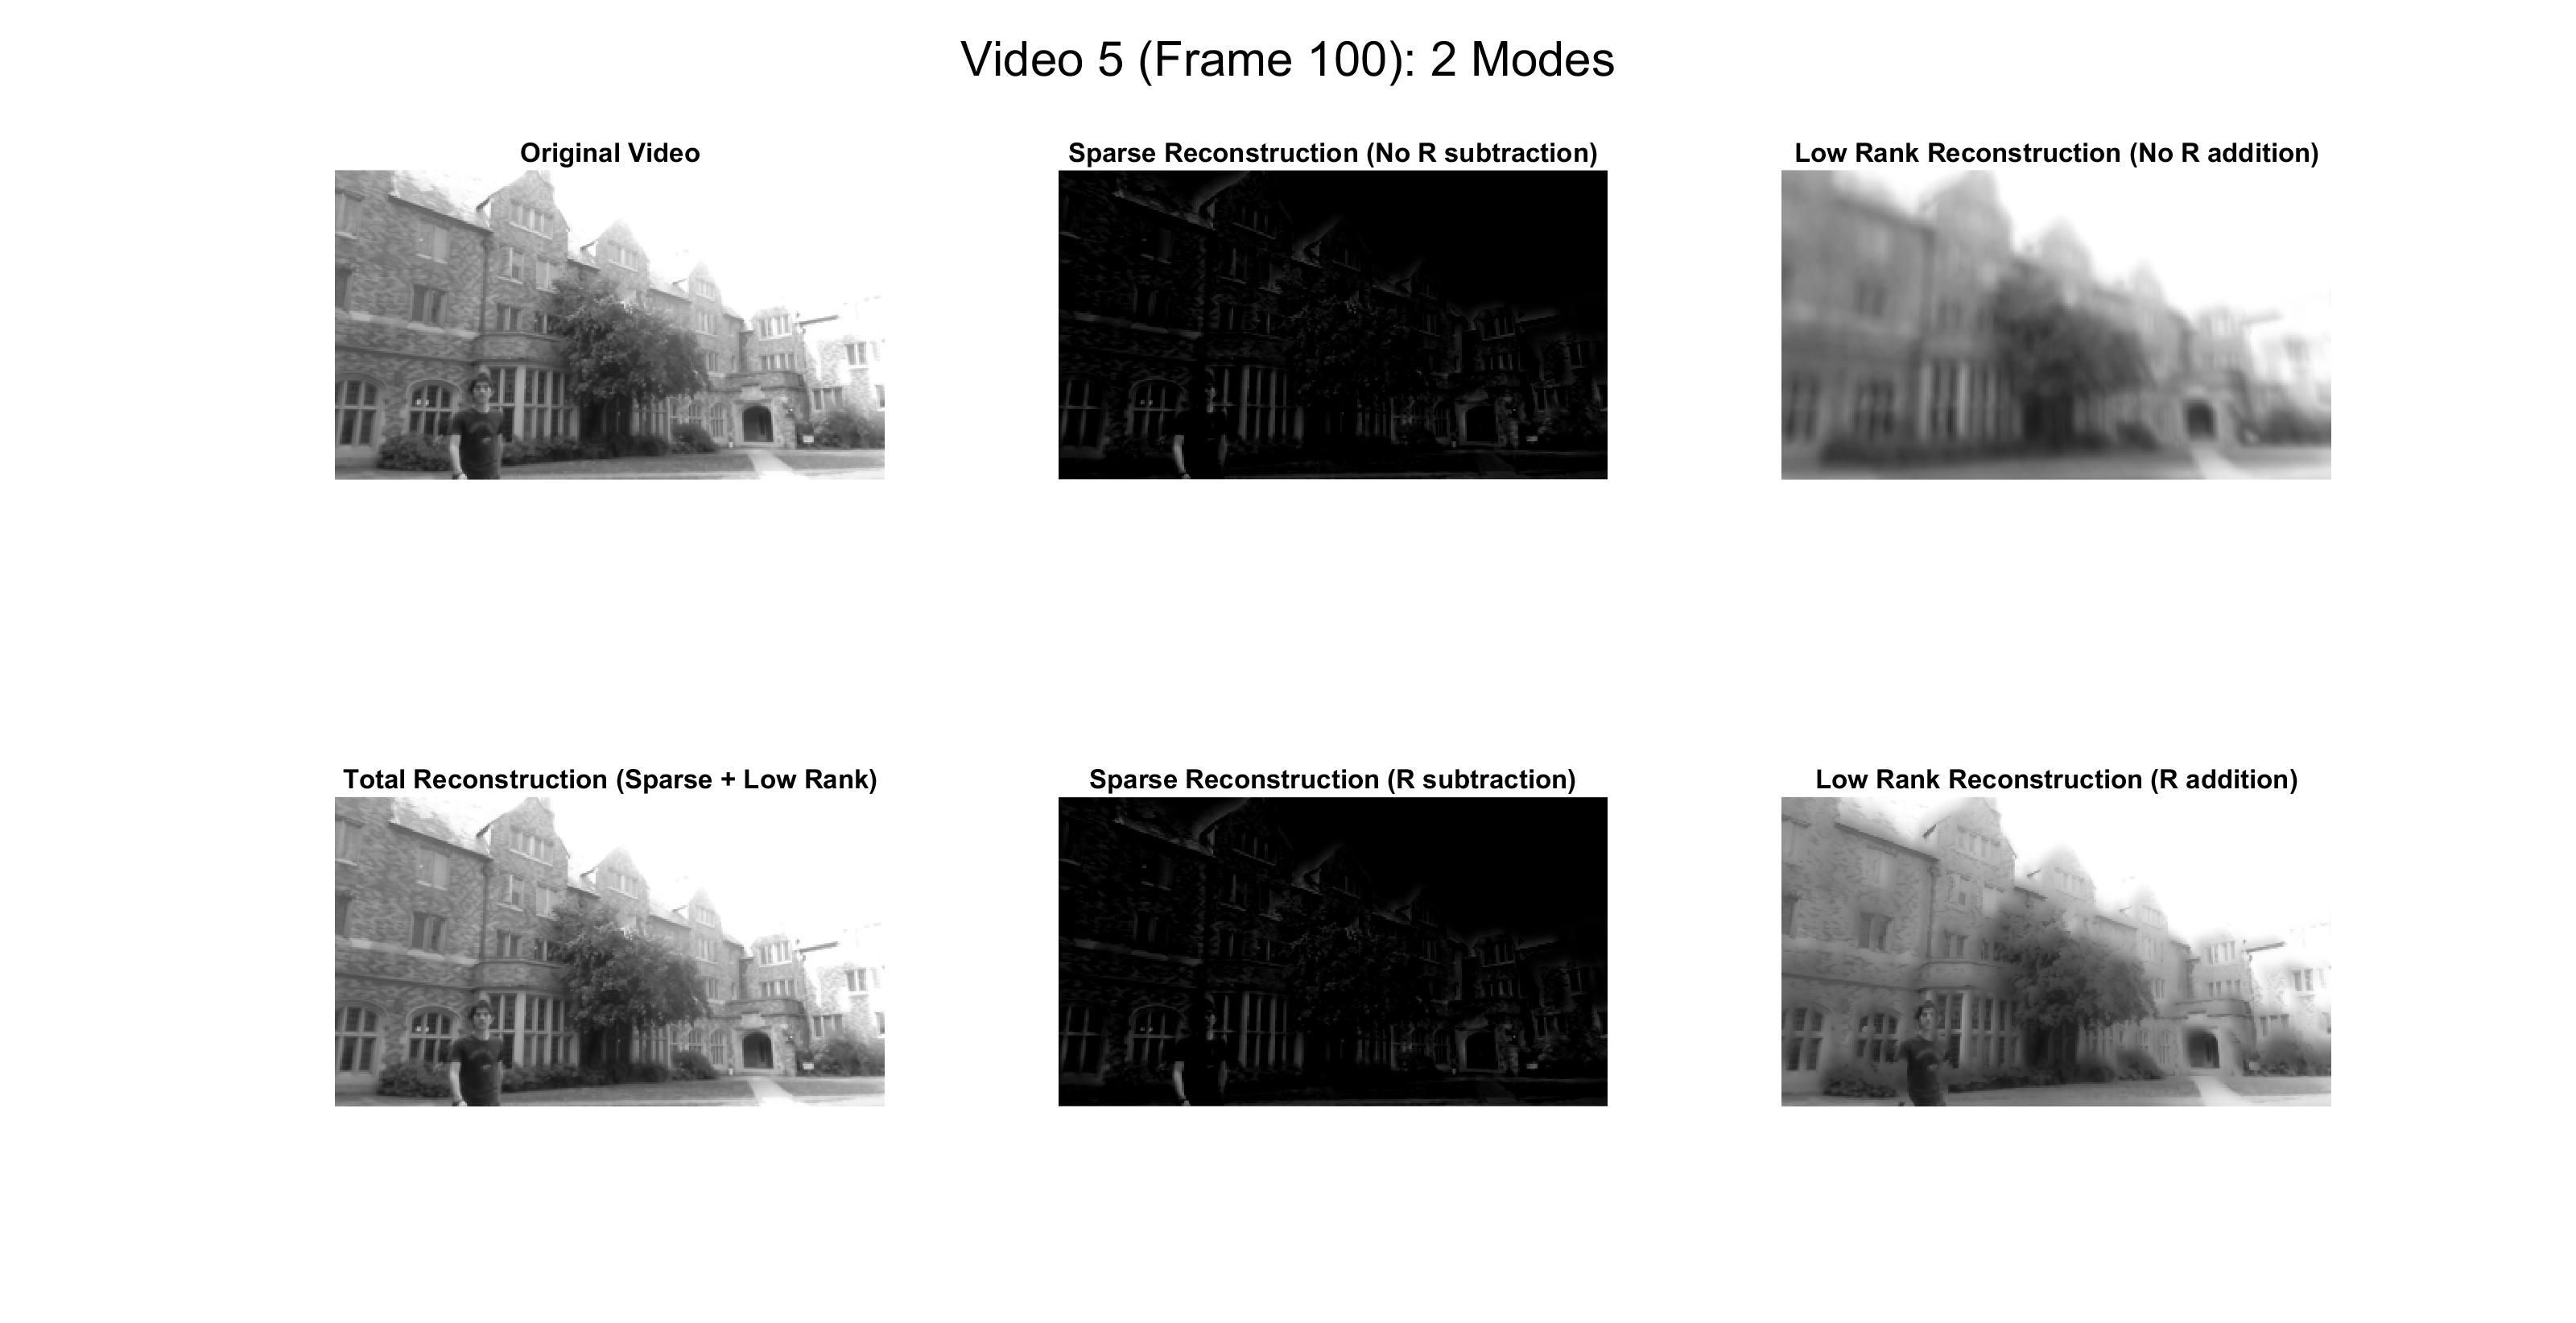
\includegraphics[width = 16cm]{vid5image}
\caption{\label{fig:scaled_diss} Video separation and reconstruction (Video 3)}
\end{center}
\end{figure}
\textbf{Video 5: Heavy Noise} \\
In this video, we introduced heavy noise to our video via intentional, large-scale shaking of the laptop (recording device). This video was recorded in the exact location of Video 4 (Light Noise) using the same foreground object (student walking around), so that we could directly compare how light and heavy noise affect the decompositions. \\ \\
We approximated that there were two significant modes from our singular value decomposition and subsequent energy plot. However, the plot of "omega" values once again confirmed that only one of these modes was important for background extraction; it was so small that it could not be visualized on the same scale as the other mode. \\ \\
In terms of image reconstruction, we see that both of our sparse reconstruction did worse at extracting the foreground, compared to Video 4 (Light Noise). The sparse reconstruction shows more of the buildings to the right, which are part of the background. Once again, although the low-rank approximation without "R" addition is significantly blurry, it successfully removes the object image from it. While the low-rank reconstruction with "R" addition has a more clear image, it leaves a significant part of the foreground object. Finally, we see that the total reconstruction matches the original video well.

\section*{\fontsize{19}{15}\selectfont Summary and Conclusions}
We recorded five sets of videos, with a moving foreground, and a static background. We performed the DMD algorithm to create a low-rank and sparse approximation of this data which represented the foreground and background of the object. We were able to do this successfully in a variety of scenarios, including two where we introduced noise to the videos. \\ \\
Overall, although the energy plots showed that there were some modes that may be significant, our plots of the actual "omega" values showed that only one mode was important to determining the background in every case. These omega values represent the eigen vectors, and a lower value means that it captures more of the background. Therefore we could have theoretically done all of these approximations by taking only the most significant mode from our singular value decomposition. We also see that across videos, it seems that videos with lower omega values had better background approximations; our videos with high noise had blurry backgrounds but still had relatively good foreground object and background separation. In addition, we found that our "R" matrix did not do particularly well - although it did not differ very much in the sparse reconstructions, when we added it to our low-rank reconstructions (represent background), it added parts of the object back, which decreased the accuracy of the foreground and background extraction. \\ \\
We did record a video in which the camera panned to somewhat follow the foreground's movement, effectively changing the background, albeit slightly. However, we did not do analysis on this video as we realized afterwards that this does not create a distinguished foreground and background; in this video, both are moving as time goes on, making them effectively both foreground objects. \\ \\
One item we did not visualize was how changing the number of modes affected the difference between the low-rank and sparse reconstructions with and without R. We found that increasing the number of modes used still lead to better background and foreground separation when we didn't use R, compared to reconstructions where we did use the R matrix. \\ \\ 
One last thing that we could have changed is the length of the video. It may have been harder to separate the foreground from the background if there was less data, i.e, if there were fewer frames in the data. It would be interesting to experimentally test how length of the video changes the decomposition and reconstruction of the videos. \\ \\
\pagebreak




\section*{\fontsize{19}{15}\selectfont Appendix A}
\subsection*{MATLAB functions used and implementation}
"abs(X)" : Returns the absolute value of every element in "X". We used this when calculating our DMD's approximate sparse reconstruction. \\ \\
"diag(X)" : Returns a column vector of the diagonal values of a matrix. We used this to generate our variance numbers from SVD. \\ \\
"double(X)" : Converts elements of "X" into type "double". We used this to convert "uint8" values into type "double" for analysis. \\ \\
"[W,D] = eig(A)" : Returns diagonal matrix "D" of eigenvalues and matrix "W" whose columns are the corresponding right eigenvectors, so that "A*V" = "V*D". We used this to find the eigen decomposition of our "Atilde" matrix. \\ \\
"imread(file)": Reads in an image file as a 3D or 2D matrix (based on if the images is color or grayscale). We used this to load in the Yale Faces for part 1. \\ \\
"implay(X)" : If "X" is a 3D matrix, plays "X" as a video, where each "(:,:,i)" slice is a timepoint to extract a matrix (therefore a frame) to display. We used this to compare original video to the separated ones. \\ \\
"imshow(X)" : Displays the matrix "X" as an image. We used this to compare frames the original video to the DMD's sparse and low-rank reconstruction frames. \\ \\
"length(A)" : Returns the length of the vector A. We used this as a parameter to reshape the data from columns back to matrices. \\ \\
"reshape(X,sz)" : Reshapes the array or matrix "X" to the size "sz". We used this to resize our image matrices from video frames into column vectors at each timepoint for data storage. We also used this to convert these column vectors back to a matrix, to view the image. \\ \\
"size(X)" : Returns the dimensions of the matrix "X". We used this to calculate the size of our matrix in our DMD algorithm. \\ \\
"[u,s,v] = svd(X)" : Returns the $U$, $S$, and $V$ matrices corresponded with the singular value decomposition of "X". We used this in our initial steps of the DMD algorithm. \\ \\
"uint8(X)" : Converts elements of "X" into type "uint8". We used this to convert our double values to uint8 to view them using "imshow". \\ \\
"VideoReader(mov.mp4)" : Creates a "VideoReader" object, with information such as frame rate and duration. We used this to load in our video files for analysis, and create our "dt" and "t" vectors. \\ \\
"zeros(X,Y)" : Creates a matrix of zeros of a specified size "X" and "Y". We used this to create an empty time dynamics matrix to iteratively fill in through a loop. \\ \\

\section*{\fontsize{19}{15}\selectfont Appendix B}
\subsection*{MATLAB code}
\begin{lstlisting}[style=Matlab-editor]
clear all; close all; clc; 

clear all; close all; clc;
    
%% Read in files (vid 1)
%Replace this with whatever movie to load in
vid1 = VideoReader('mov5.mp4');
dt = 1/vid1.Framerate;
t = 0:dt:vid1.Duration;
vidFrames = read(vid1);
numFrames = get(vid1,'numberOfFrames');
%% Load
for k = 1 : numFrames
    mov(k).cdata = vidFrames(:,:,:,k);
    mov(k).colormap = [];
end

fdata = [];
for j=1:numFrames
    X=frame2im(mov(j));
    
    fdata = [fdata, reshape(double(rgb2gray(imresize(X, 0.25))), [180*320,1])];
    %imshow(imresize(X, 0.25)); drawnow
end

%%  DMD
%%%%%% body of DMD %%%%%%%%%%
X1 = fdata(:,1:end-1); 
X2 = fdata(:,2:end);

[U,S,V] = svd(X1, 'econ');

subplot(1,2,1)
plot(diag(S)/sum(diag(S)), 'bo', 'Linewidth', 2, 'MarkerSize', 10, 'MarkerFaceColor', 'g');
title("Energies of Singular Values", 'Fontsize', 24); ylabel("Energy Captured"); xlabel("Singular Values");
grid on

r = 2;

U_r = U(:, 1:r); % truncate to rank-r
S_r = S(1:r, 1:r);
V_r = V(:, 1:r);
Atilde = U_r' * X2 * V_r / S_r; % low-rank dynamics
[W_r, D] = eig(Atilde);
Phi = X2 * V_r / S_r * W_r; % DMD modes

lambda = diag(D); % discrete-time eigenvalues
omega = log(lambda)/dt; % continuous-time eigenvalues

subplot(1,2,2)
bar(abs(omega), 'm')
title("Omega Values (Absolute Value)",'Fontsize', 24);
set(gca,'XTick',[]); xlabel("Omegas"); ylabel("Absolute Value of Omegas");
grid on
%% Compute DMD mode amplitudes b
x1 = X1(:, 1);
b = Phi\x1;

%% DMD reconstruction
mm1 = size(X1, 2); % mm1 = m - 1
time_dynamics = zeros(r, mm1);
t = (0:mm1-1)*dt; % time vector
for iter = 1:mm1,
time_dynamics(:,iter) = (b.*exp(omega*t(iter)));
end;
Xdmd = Phi * time_dynamics;

%% Create Sparse and Nonsparse

Xsparse = X1 - abs(Xdmd);

R = Xsparse.*(Xsparse<0);

X_bg = R + abs(Xdmd);
X_fg = Xsparse - R;

X_reconstructed =  X_fg + X_bg;

%% Display
temp1 = reshape(Xsparse, [180,320, length(t)]);
temp2 = reshape(Xdmd, [180,320,length(t)]);
temp3 = reshape(X_bg, [180,320,length(t)]);
temp4 =  reshape(X_fg, [180,320,length(t)]);
temp5 =  reshape(X_reconstructed, [180,320,length(t)]);
temp6 =  reshape(X1, [180,320,length(t)]);
temp7 = reshape(R, [180,320,length(t)]);

% implay(uint8(temp3));
% imshow(uint8(temp3(:,:,100)))
% imshow(uint8(temp3(:,:,100)))
% imshow(uint8(temp3(:,:,100)))

%% Plotting
figure()
framenum = 100;

subplot(2,3,1)
imshow(uint8(temp6(:,:,framenum)))
title("Original Video");

subplot(2,3,2)
imshow(uint8(temp1(:,:,framenum)))
title("Sparse Reconstruction (No R subtraction)");


subplot(2,3,3)
imshow(uint8(temp2(:,:,framenum)))
title("Low Rank Reconstruction (No R addition)");

subplot(2,3,6)
imshow(uint8(temp3(:,:,framenum)))
title("Low Rank Reconstruction (R addition)");

subplot(2,3,5)
imshow(uint8(temp4(:,:,framenum)))
title("Sparse Reconstruction (R subtraction)");

subplot(2,3,4)
imshow(uint8(temp5(:,:,framenum)))
title("Total Reconstruction (Sparse + Low Rank)");

sgtitle(strcat("Video 5 (Frame ", int2str(framenum), "): ", int2str(r)," Modes"), 'Fontsize', 20)
\end{lstlisting}
\end{document}
